
  % NEW STRUCTURE

  % Chapter: Methods

  %  1. Experimental Environment
  %      * 1.1. Computational Infrastructure
  %      * 1.2. CARLA Simulation Environment


  %  2. Datasets and Preprocessing
  %      * 2.1. Self-Driving Dataset Generation
  %      * 2.2. Benchmark Datasets (CIFAR-10, MNIST)
  %      * 2.3. Dataset Variants and Perturbations
  %          * 2.3.1. The Perturbed MNIST (PMNIST) Dataset
  %          * 2.3.2. Other MNIST Variants
  %          * 2.3.3. Noise Perturbation Methods

  %  3. Model Architectures
  %      * 3.1. Convolutional Neural Networks (CNN)
  %      * 3.2. Vision Transformers (ViT)
  %      * 3.3. Vision-Language Models (VLM)


  %  4. Model Training and Fine-Tuning
  %      * 4.1. CNN Training
  %      * 4.2. ViT Training and Fine-Tuning
  %      * 4.3. VLM Fine-Tuning for Steering Prediction


  %  5. Evaluation and Analysis Methods
  %      * 5.1. Network Evaluation Setups (Single, Dual, and Remote Environments)
  %      * 5.2. Regression-to-Classification Transformation
  %      * 5.3. Uncertainty Quantification via Softmax Clustering
  %      * 5.4. Image Distance Metrics for Robustness Analysis
  %      * 5.5. Zero-Shot VLM Evaluation on CIFAR-10


% TODO METHODS
% NEED TO ADD FIGURES TO AVOID COGNITIVE OVERLOAD
% EXAMPLES OF DATASETS
% CARLA FIGURE OF 8
% EXAMPLE PROMPTS in verbatim macros
% EXAMPLE OF SOFTMAX OUTPUT
% EXAMPLE OF ADDED NOISE e.g. pixelation
% NEED TO ADD LANE INVASION CONTEXT i.e. 0.85 ud away from  path

% More Todos
% Re-use 03-Methods-04-llm-driven-carla.tex for prompting examples
% Re-use 03-Methods1.tex if there is anything worth using (VLM Methods)
% In this .tex file, there is a section that covers VLMs, though 03-Methods1.tex at first
% sight seems to have plenty of detail which in turn has to be examined to see if it best
% fits in methods or results


%%%%%%%%%%%
% METHODS %
%%%%%%%%%%%

\chapter{Methods}
\label{methods_final}

This section describes the methods used to develop and validate distance-based safety assessment for autonomous systems. Methods cover computational infrastructure, simulation environment, distance metrics, noise perturbation, dataset generation, neural network architectures, training protocols, softmax clustering algorithm, regression-to-classification transformation, and Vision Language Model implementation.

%%%%%%%%%%%%%%%%%%%%%%%%%%%%%%%%%%%%%%%%
% IMPLEMENTATION PLATFORM AND HARDWARE %
%%%%%%%%%%%%%%%%%%%%%%%%%%%%%%%%%%%%%%%%

\section{Experimental Infrastructure}
\label{methods:hardware}

All code implementations were developed in Python (\cite{python}) using standard libraries (NumPy, OpenCV, Matplotlib) with shell scripting for batch job execution on the City St George's, University of London, School of Science and Technology HPC (high-performance computing cluster). The remote compute infrastructure comprised 19 GPU cards across five nodes with a total of 872GB GPU memory, where a maximum of 8 GPU cards from the pool were used concurrently. A local workstation was used for code development, network training and testing, as  well as running the CARLA simulator (\cite{dosovitskiy17}). GitHub (\cite{github}) was used as the code repository.

\begin{longtable}{@{}lcc@{}}
\toprule
Node & GPU Configuration & Total Memory \\
\midrule
\endfirsthead
\toprule
Node & GPU Configuration & Total Memory \\
\midrule
\endhead
gpu01 & 3 × Quadro RTX 8000 & 138GB \\
gpu02 & 8 × NVIDIA A100-PCIE-40GB & 320GB \\
gpu03 & 2 × NVIDIA A100 80GB PCIe & 160GB \\
gpu04 & 4 × NVIDIA A100 80GB PCIe & 320GB \\
gpu05 & 2 × NVIDIA A100 80GB PCIe & 160GB \\
\midrule
\textbf{Total} & \textbf{19 cards} & \textbf{872GB} \\
\bottomrule
\caption{CSGULSST HPC GPU Infrastructure}
\label{tab:hpc_hardware}
\end{longtable}

The local development workstation utilized a GeForce GTX 1060 6GB later upgraded to an RTX 3060 12GB.

\begin{longtable}{@{}lcc@{}}
\toprule
Configuration & GPU Model & Memory \\
\midrule
\endfirsthead
\toprule
Configuration & GPU Model & Memory \\
\midrule
\endhead
Initial Setup & GeForce GTX 1060 & 6GB \\
Upgraded Setup & GeForce RTX 3060 & 12GB \\
\bottomrule
\caption{Local Development Workstation GPU Configuration}
\label{tab:local_hardware}
\end{longtable}

%%%%%%%%%%%%%%%%%%%
% CARLA SIMULATOR %
%%%%%%%%%%%%%%%%%%%
\section{CARLA Simulator}
\label{methods:carla}

\begin{figure}[h]
\centering
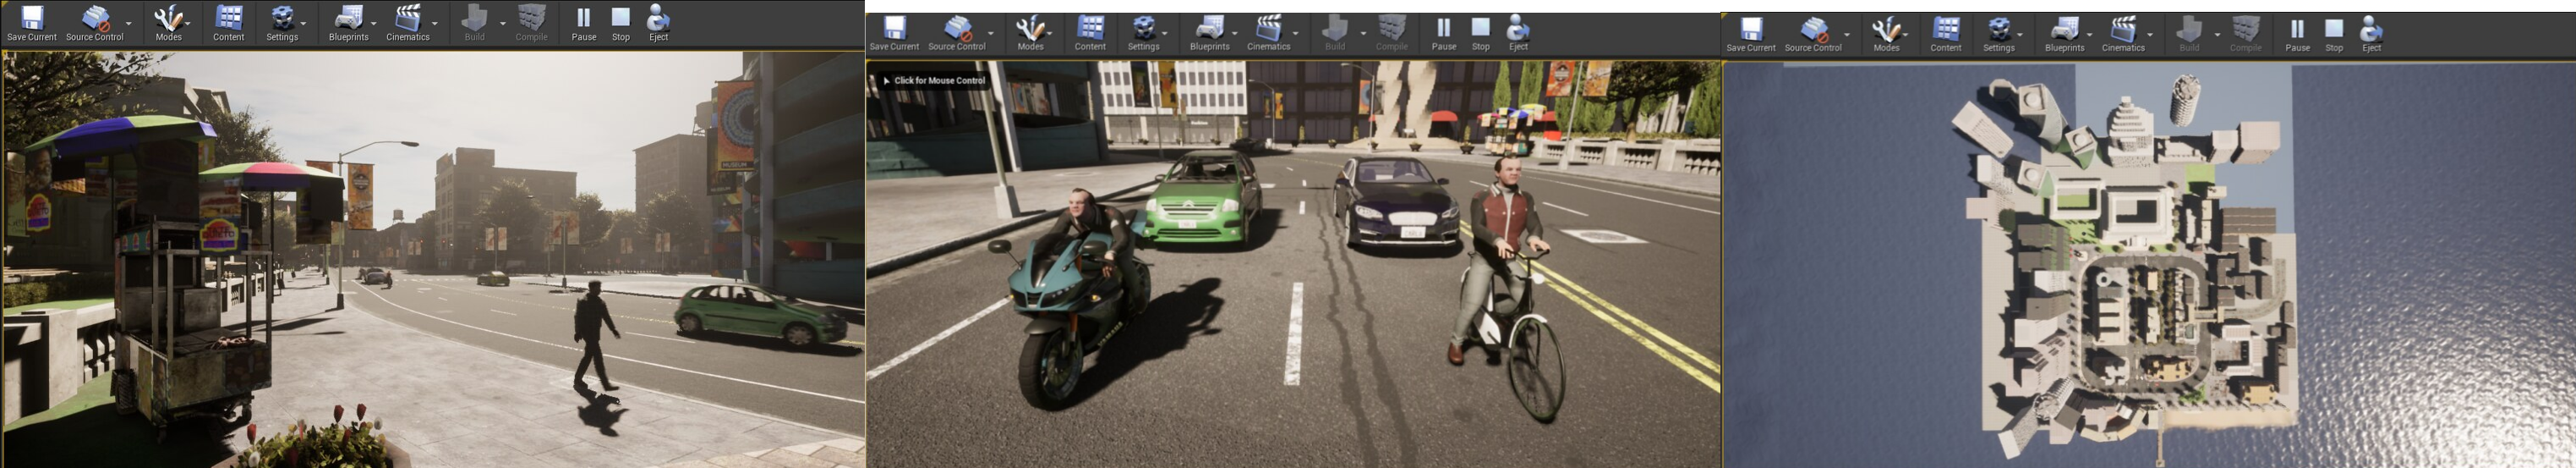
\includegraphics[width=0.99\textwidth]{Figures/Methods/CarlaTown10.png}
\caption{From left to right, left: a running simulation in the CARLA Town10 map, with 60 vehicles and 100 pedestrians. Middle: is a similar simulation, motorcyclist, cyclist and two vehicles waiting at a set of traffic ligths and right: a bird's eye view of CARLA Town10 map.}
\label{fig:CarlaTown10}
\end{figure}

CARLA (Car Learning to Act) is a open-source simulator (Figure \ref{fig:CarlaTown10}) for autonomous driving research, built on Unreal Engine (\cite{unrealengine}). CARLA (Car Learning to Act) is a open-source simulator for autonomous driving research, built on Unreal Engine. The Python API provides a client-server architecture where the client establishes a TCP connection to the simulator instance. The client retrieves the world object representing the simulation environment and can access various components for controlling autonomous behaviour. World settings can be modified to enable synchronous or asynchronous execution modes, with synchronous mode providing deterministic simulation steps through world tick calls. The API exposes a blueprint library system for actor spawning, where vehicle and pedestrian blueprints are filtered and configured with attributes such as colour and driver appearance. Vehicles and pedestrians can be spawned at spawn points, which in turn are retrieved from the world's navigation mesh. The simulation loop maintains real-time execution through continuous world ticking. Weather conditions including cloudiness, precipitation, wind intensity, fog density, and surface wetness can be dynamically controlled. Solar positioning is adjustable through azimuth and altitude angles. The framework supports autonomous driving agents which were not used, a custom agent was built for this study. 

% It supports the full autonomous vehicle (AV) development lifecycle, from algorithm prototyping to system validation, offering a safe, scalable alternative to costly and risky real-world testing. Its client-server architecture ensures flexibility, with a Python/C++ API enabling precise control over sensors, weather, actors, and custom maps via the OpenDRIVE (\cite{opendrive}) standard. Synchronous mode guarantees deterministic, repeatable experiments critical for scientific rigor, while asynchronous mode suits real-time exploration. CARLA’s Actor-Blueprint system allows dynamic spawning of vehicles, pedestrians, and sensors, with configurable attributes for tailored scenarios. 

\subsection{Generating training datasets with CARLA}
\label{methods:carla_gen_train_datasets}
The training dataset generation process operates through automated CARLA simulation runs. To define a route, a set of pre-defined waypoints, retrievable from the town map mesh, are examined. A waypoint has road\_id and lane\_id attributes. The figure of 8 express way around Town04 map (Figure \ref{fig:Town04FigureOfEight}) can be identified by selecting road\_ids with 4 lane\_ids, then ordering the road\_ids in a list that will that will result in the desired sequence of waypoints. A vehicle is spawned at the first waypoint of the sequence with an RGB camera mounted at a configurable position and orientation.
The simulated vehicle follows the road waypoint sequence along 28 road\_id segments, using waypoints at 1 unit of distance intervals (for regression and 15 bin quantized classification) and 3 units of distance intervals (5 and 3 bin quantized classification). Permanent waypoint lines are drawn for lane segmentation. The steering algorithm computes the angular difference between the vehicle's transform orientation and the nearest waypoint's transform orientation. This delta is applied as a steering correction to align the vehicle path with the road centre line.

\begin{figure}[h]
\centering
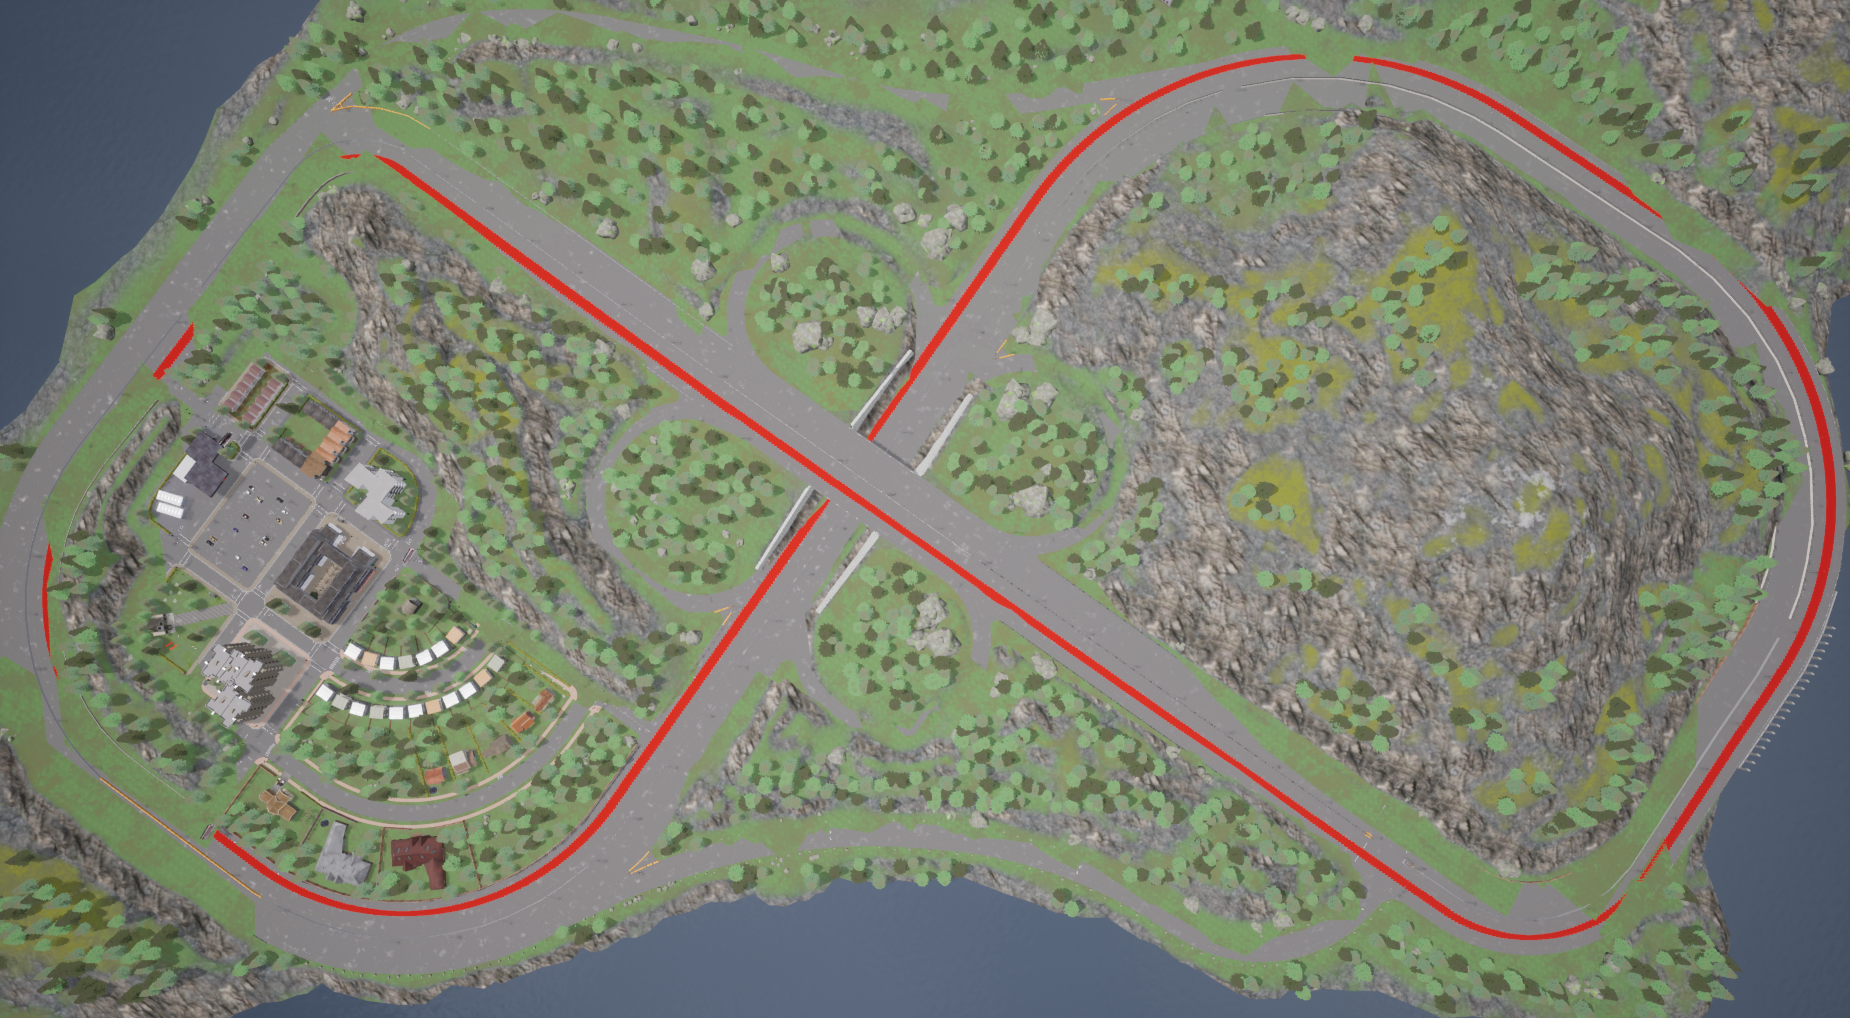
\includegraphics[width=0.99\textwidth]{Figures/Methods/Town04FigureOfEight.png}
\caption{The CARLA Town04 Figure-of-eight circuit. The path is set on lane id -2, that is the second from left to right, on the right hand lane. The circuit is composed by determining which road sections comprise the desired route, then concatenating the waypoints of each section sequentially to form a full lap.}
\label{fig:Town04FigureOfEight}
\end{figure}

Two dataset generation modes we developed for this study: continuous regression mode saves the raw steering angle delta (steering adjustment from one waypoint to the next) as the label, while quantized classification mode approximates and truncates the continuous delta to the nearest of 15, 5 or 3, as the case may be, predefined bin values ranging from -0.065 to 0.065 in CARLA's normalized control space, corresponding to approximately -+4.5 degrees of the vehicle's -+70 degree steering range \href{https://www.youtube.com/watch?v=cg6hhrpsc5g}{(video)}, noting the interval -+4.5 degrees is sufficient to steer the vehicle around the circuit without lane invasions.
Data collection occurs at each simulation tick, capturing RGB images with steering angles embedded in timestamped filenames e.g. 20250314\_094117\_214470\_steering\_-0.0167.jpg (steering value -0.0167 corresponds to -1.17 degrees, that is vehicle is steering slightly left) such that alphabetical order will correspond to the order image file was generated. Ground truth safety distances are computed as perpendicular distances from vehicle position to the lane centre line defined by consecutive waypoint pairs. Orthogonal distances from the centre line exceeding 0.85 units indicate lane invasion events. Each complete figure of eight lap generates approximately 28,000 labelled images under synchronous mode execution.

\begin{figure}[h!]
\centering
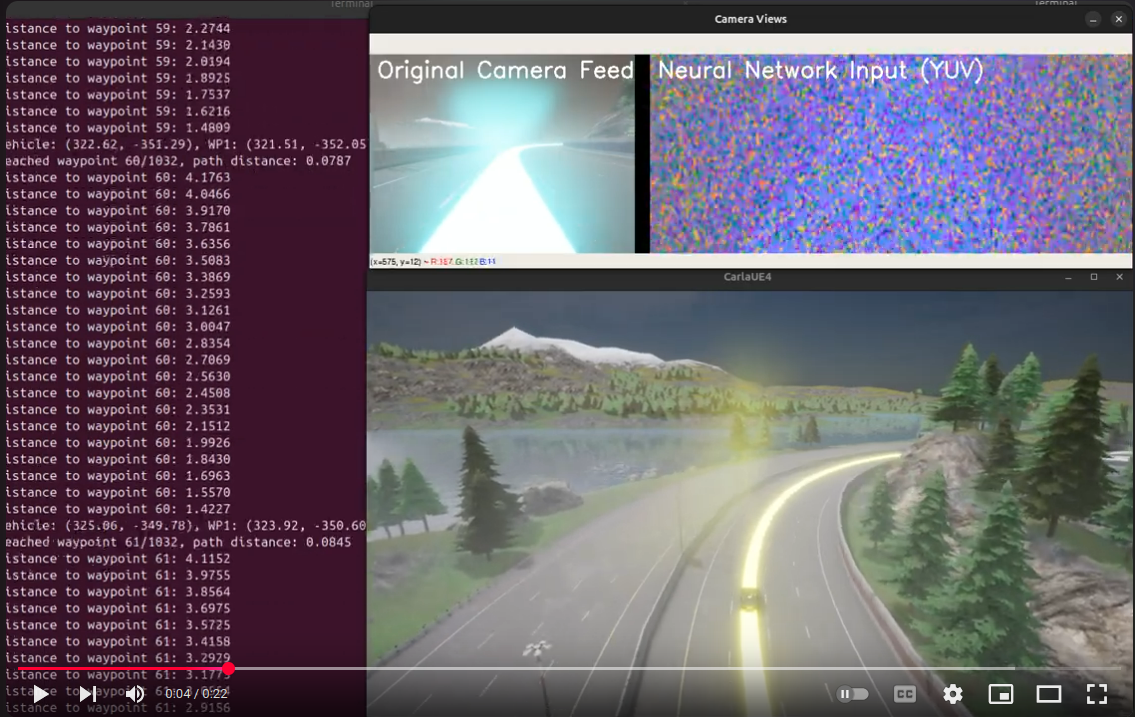
\includegraphics[width=0.99\textwidth]{Figures/Results/youtubeidCzJlbYX0CnQ_experiment239_30pc_pepper_noise_5bin_cnn_balanced.png}
\caption{A CARLA simulation where the vehicle is driven by a CNN trained on a 5 bin balanced dataset, and subject to 30\% pepper noise. The column on the left are debug prints of distances to the nearest waypoints, virtual anchors and part of a mesh in the CARLA world when actors e.g. vehicles and pedestrians, can be spawned/created/instantiated, the larger figure on the bottom left is the simulator from the "spectator" perspective. The spectator is this case is set to track the vehicle at every "tick", that is, every update of the CARLA world, where spectator is set 35 units of distance along the x axis (behind the vehicle) and 20 units of distances along the z axis (above the simulated vehicle), while the pitch (rotation along the lateral axis) set to -15 degrees, that is the spectator is looking down. There is no translation along the y axis, and no rotation along the vertical axis (yaw) or longitudinal axis (roll). The image on the top left of the simulator is the one frame capture from front facing vehicle camera and the image on the top right is the camera image cropped to exclude the section above the horizon and resized to 200w x 66h pixels, then moved from RGB to YUV space.}
\label{fig:youtubeidCzJlbYX0CnQ_experiment239_30pc_pepper_noise_5bin_cnn_balanced}
\end{figure}


%%%%%%%%%%%%%%%%%%%%%%%%%%%%%%%%%%%
% DISTANCE METRICS: BD, HI and KL %
%%%%%%%%%%%%%%%%%%%%%%%%%%%%%%%%%%%

\section{Image Distance Metrics}
\label{methods:distance_metrics}

Three statistical distance metrics are employed to quantify distances between original and noise-corrupted images: Bhattacharyya Distance, Histogram Intersection, and Kullback-Leibler (KL) Divergence. 

The Bhattacharyya Distance (\cite{bhattacharyya1943}) is a statistical measure used to quantify the similarity between two probability distributions. It provides a way to measure the amount of overlap between two statistical samples or populations, indicating how "close" they are to each other in a statistical sense.

Histogram Intersection (\cite{swain1991}) is a method used in computer vision to compare the similarity of two images. It operates by measuring the overlap between two colour histograms, effectively counting the number of pixels from a model that have corresponding pixels of the same colour in a target image. 

The Kullback-Leibler Divergence (\cite{kullback1951}) is a measure from information theory that quantifies how one probability distribution differs from a second, reference distribution. It is used to calculate the information lost when an approximate model is used to represent a true distribution, effectively measuring their dissimilarity. 

Standard formulations are adapted for multi-channel RGB images by computing histogram-based representations for each colour channel. Bhattacharyya Distance and KL Divergence increase as dissimilarity increases, while Histogram Intersection decreases as dissimilarity increases.

For RGB images treated as histogram distributions with ground truth and corrupted bin counts $P,Q$ respectively, the total pixel count is:
\begin{equation}
\label{eq:t_p}
  t_p = \prod\limits_{n=1}^{N}I_n   
\end{equation}
where $N$ is the number of image dimensions and $I_n$ is the number of elements in dimension $n$.

\textbf{Bhattacharyya Distance} is defined as the negative logarithm of the Bhattacharyya coefficient:
\begin{equation}
    D_{B}(P,Q) = -\ln(BC(P,Q))
\end{equation}
where for multi-channel RGB:
\begin{equation}
BC(P,Q) = \sum\limits_{x\in \mathcal{X}} \frac{\sqrt{P(x)Q(x)}}{t_p}
\end{equation}

\textbf{Kullback-Leibler Divergence} for RGB images:
\begin{equation}
 D_{KL}(P \parallel Q) = \sum\limits_{x\in\mathcal{X}} \frac{P(x)}{t_p} \log\left(\frac{P(x)+\epsilon}{Q(x)+\epsilon}\right)
\end{equation}

We add a small positive term $ \epsilon $ to $ P(x), Q(x) $ to avoid division by zero, and also to avoid taking the logarithm base 10 of zero which is undefined.

We note that the KL Divergence in addition to, for our purposes, being fragile, is also asymmetric. that is the divergence from P to Q is not the same as the divergence from Q to P.

Note we use discrete rather than the continuous values. That is, we use the original byte value for each channel and the discrete relative entropy equation. If we convert the distribution to a PDF, that is, with all aggregated counts summing to one, we would use the continuous equation. The PDF seems like the better way to go as it is a normalised value, though if we are dealing with a known network, the input is always of the same the same dimensions and can be considered normative, that is the RGB mean is constrained by, and bound to, the input size.

\textbf{Histogram Intersection} for RGB distributions:
\begin{equation}
  H_{I}(P, Q) = \frac{1}{t_p} \sum\limits_{x\in\mathcal{X}}\min(P(x), Q(x))   
\end{equation}

If $P,Q$ are the same for every $ x $, then the summation will be equal to the product $t_p$, resulting in 1, meaning there is a complete overlap between the two distributions. If $argmin(P(x), Q(x))$ is equal to zero for every $x$, then the summation will be equal to zero meaning there is no overlap between the histograms.

Since the histogram RGB intersection does not take square roots or logs, it is the most computationally efficient of the three distance metrics we investigate.

%%%%%%%%%%%%%%%%%%%%%%%%%%%%%
% NOISE PERTURBATION METHODS %
%%%%%%%%%%%%%%%%%%%%%%%%%%%%%
\section{Noise Perturbation Methods}
\label{methods:noise_perturbation}

Twelve distinct noise perturbation types are applied to MNIST training images to simulate real-world degradation conditions and evaluate model robustness, based on \cite{hendrycks2019benchmarking}. Each perturbation type operates across ten intensity levels designed to produce approximately-linear accuracy degradation from near 100\% accuracy (level 0) to average 50\% (level 10). All perturbations operate on grayscale images with pixel values normalized to the range $[-1, 1]$.

Parameter values for each perturbation type and intensity level were determined through trial-and-error, adjusting parameters until the linear degradation profile was approximated.

The twelve perturbation types are:

\textbf{Brightness} adjusts global illumination by adding constant values ranging from 0.1 to 1.0 across intensity levels. Higher values simulate overexposure conditions.

\textbf{Contrast} modifies pixel intensity relationships relative to the image mean. Positive values (3.0 to 0.2) increase contrast while negative values (-0.2 to -0.6) reduce contrast, simulating poor lighting conditions.

\textbf{Defocus Blur} applies uniform convolution kernels of varying sizes (3×3 to 8×8) with blur amounts from 0.1 to 1.5, simulating camera focus issues.

\textbf{Fog} creates atmospheric scattering effects using Gaussian distance-based masks with fog levels and densities ranging from 0.1 to 0.6, simulating reduced visibility conditions.

\textbf{Frost} generates crystalline patterns through thresholded Gaussian noise (levels 6 to 18) followed by Gaussian blurring with 5×5 kernels, simulating ice formation on camera lenses.

\textbf{Gaussian Noise} adds normally distributed random values with means from 0.05 to 0.87 and fixed standard deviation of 0.25, simulating sensor thermal noise.

\textbf{Impulse Noise} introduces salt-and-pepper artifacts by randomly setting pixel values to maximum intensity, with density ranging from 0.25 to 0.75, simulating sensor dead pixels.

\textbf{Motion Blur} applies directional convolution kernels of increasing size (1×1 to 10×10) at 0° angle, simulating camera or subject movement.

\begin{figure}[h]
\centering

\includegraphics[width=0.99\textwidth]{Figures/Methods/Pixelation_Digit_5_1_to_10_intensity.png}
\caption{MNIST Digit 5 subject to 10 levels of pixelation from left to right.}
\label{fig:Pixelation_Digit_5_1_to_10_intensity}
\end{figure}

\textbf{Pixelation} (Figure \ref{fig:Pixelation_Digit_5_1_to_10_intensity}) reduces spatial resolution through downsampling by factors from 0.7 to 5.7 followed by nearest-neighbor upsampling, simulating low-resolution capture conditions.

\textbf{Shot Noise} introduces Poisson-distributed noise with intensities from 0.1 to 0.57, simulating photon counting limitations in low-light conditions.

\textbf{Snow} creates precipitation effects by randomly placing high-intensity pixels (snow levels 0.81 to 0.99) followed by Gaussian blurring, simulating weather-related occlusion.

\textbf{Zoom Blur} applies radial blur kernels of increasing size (1×1 to 8×8) with unit strength, simulating rapid focal length changes or camera shake.

All perturbation implementations use OpenCV (\cite{opencv}) for image processing operations.

% \cite{hendrycks2019benchmarking} introduced datasets ImageNet-C and ImageNet-P, to evaluate the robustness of image classifiers against common, non-adversarial image alterations.

% ImageNet-C is designed to test model robustness against static corruptions. It is generated by taking the 50,000 images from the standard ImageNet (ILSVRC 2012) validation set and applying 15 different types of algorithmic corruptions. These fall into categories of noise, blur, weather, and digital effects, with each corruption applied at five distinct levels of severity, resulting in a test set containing 3,750,000 images. A smaller version named Tiny ImageNet-C was also created, which applies a similar process to the Tiny ImageNet dataset, resulting in a test set of 750,000 images.

% ImageNet-P provides sequential perturbations, consisting of short, video-like sequences generated for each of the 50,000 ImageNet validation images. For each base image, 10 different types of perturbations are applied sequentially over more than 30 frames, creating a large dataset of over 15 million images designed to assess a model's stability against persistent, evolving changes.

% Table \ref{tab:imagenet_robustness_datasets} summary of these datasets.

% \begin{longtable}{@{}lccc@{}}
% \toprule
% Dataset Name & Size Calculation & Total Images & Type \\
% \midrule
% \endfirsthead
% \toprule
% Dataset Name & Size Calculation & Total Images & Type \\
% \midrule
% \endhead
% Tiny ImageNet-C (Test Set) & 10k Imgs $\times$ 15 Corrs $\times$ 5 severities & 750,000 & Static \\
% ImageNet-C & 50k Imgs $\times$ 15 Corrs $\times$ 5 severities & 3,750,000 & Static \\
% ImageNet-P* & 50k Imgs $\times$ 10 Perbs $\times$ >30 Frms & >15,000,000 & Sequential \\
% \midrule
% \bottomrule
% \caption{ImageNet Robustness Benchmark Sizes. *ImageNet-P consists of sequential image data.}
% \label{tab:imagenet_robustness_datasets}
% \end{longtable}

%%%%%%%%%%%%%%%%%%%%%%%%%%%%%
% DATASETS & DATA GENERATION %
%%%%%%%%%%%%%%%%%%%%%%%%%%%%%
\section{Datasets and Data Generation}
\label{methods:datasets}
This section describes the datasets used in this research.

\subsection{CIFAR-10 and MNIST}

\begin{figure}[h]
\centering
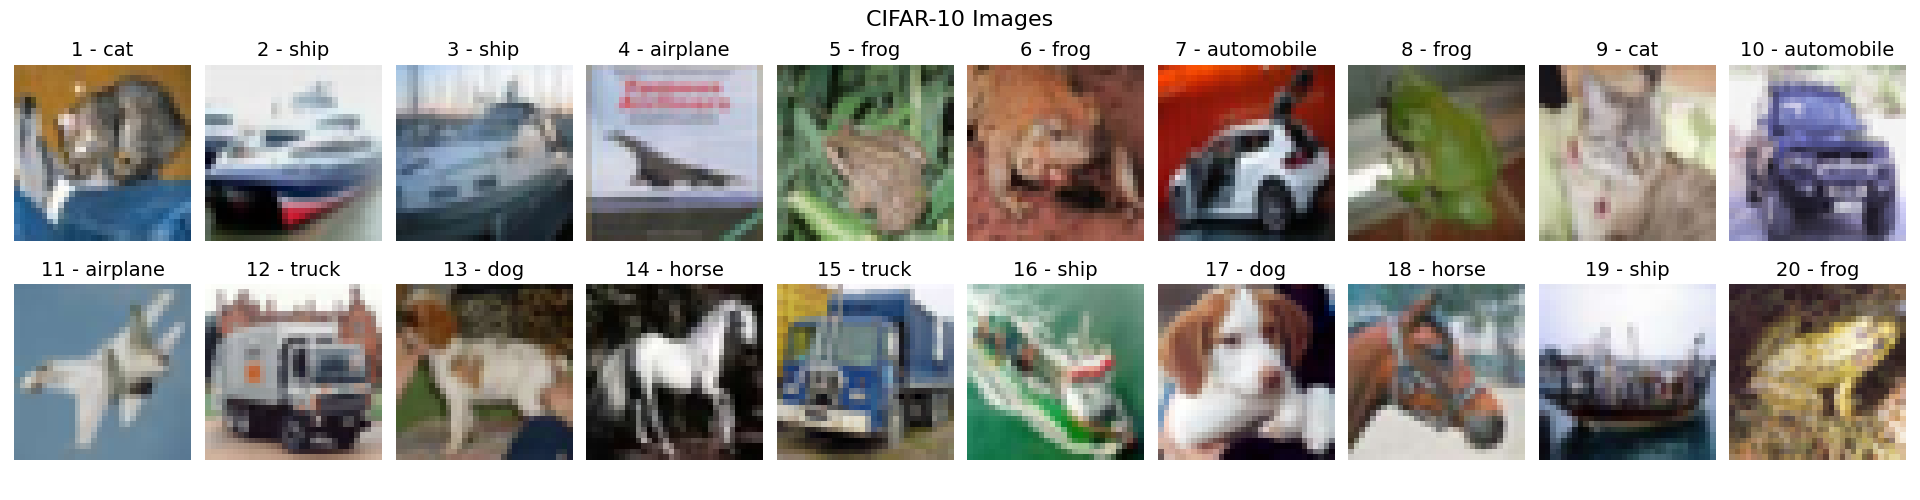
\includegraphics[width=0.99\textwidth]{Figures/Methods/CIFAR-10-Images-20imgs-2rows-10cols.png}
\caption{Examples of the CIFAR-10 dataset classes.}
\label{fig:Images-20imgs-2rows-10cols}
\end{figure}

The MNIST dataset (\cite{mnist}) is a collection of 70,000 (60k training, 10k testing) grayscale handwritten digit images (0-9), widely used for image classification benchmarking. It comprises 60,000 training images and 10,000 test images, each 28x28 pixels and is widely used for testing machine learning models. CIFAR-10 (\cite{cifar10}) consists of 60,000 (50k training, 10k testing) colour images (32x32 pixels) across 10 classes, like airplanes, cats, and trucks as shown in Figure \ref{fig:Images-20imgs-2rows-10cols}. It has 50,000 training images and 10,000 test images. 

\subsection{The PMNIST (Perturbed MNIST) dataset}

\begin{figure}[h]
\centering
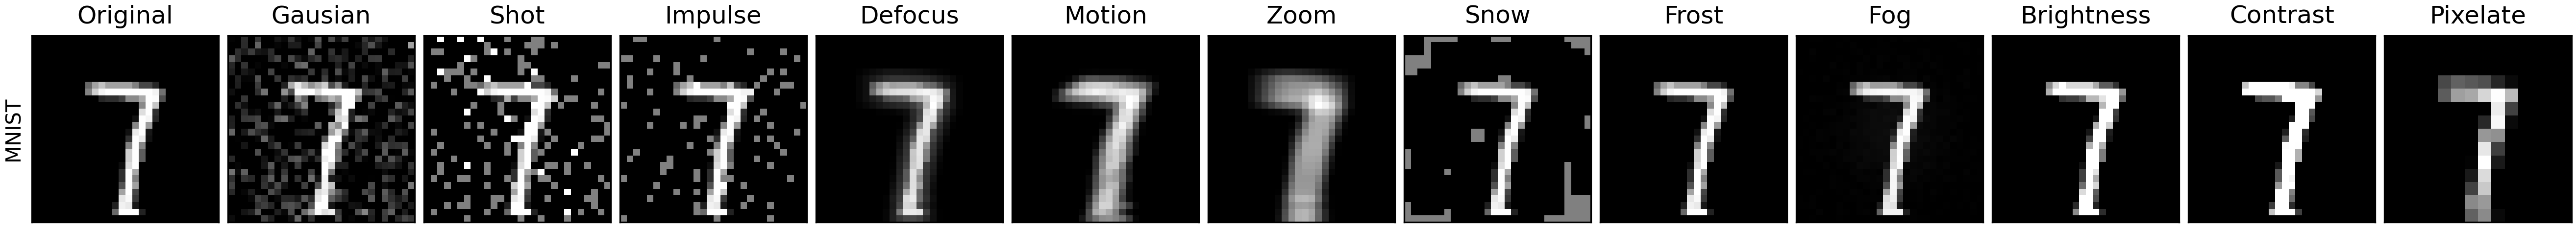
\includegraphics[width=0.99\textwidth]{Figures/Methods/MNIST_Perturbations.png}
\caption{Examples of the Perturbed MNIST - PMNIST dataset.}
\label{fig:MNIST_Perturbations}
\end{figure}

This subsection describes how the Perturbed MNIST dataset (Figure \ref{fig:MNIST_Perturbations}) was created, to help study the effect of noise on a neural network classifier predictive accuracy. We start by extending the previously described MNIST dataset, as it forms the basis of the PMNIST dataset.
The MNIST dataset, a cornerstone in the field of machine learning, serves as a benchmark for evaluating the performance of algorithms in the domain of handwritten digit recognition. Comprising a collection of 70,000 grayscale images, each of 28x28 pixel resolution, the dataset is divided into two distinct sets: a training set containing 60,000 examples, and a test set with 10,000 examples (\cite{lecun1998gradient}). Each image within the dataset is associated with a label from 0 to 9, corresponding to the digit it represents.

This dataset has been instrumental in facilitating advancements in machine learning, particularly in the development and evaluation of algorithms capable of performing classification tasks. Its widespread adoption can be attributed to several factors, including the simplicity of the task it presents and its suitability for use in benchmarking the performance of various learning algorithms, ranging from simple linear classifiers to more complex deep learning models.

A key feature of the MNIST dataset is its pre-processing stage, where the digits have been size-normalized and centered in a fixed-size image. This pre-processing reduces the variability unrelated to digit identity, allowing researchers to focus on the algorithmic challenge of digit recognition rather than on the preprocessing steps.

% The significance of the MNIST dataset in the realm of machine learning research is well-documented, with \cite{lecun1998gradient} providing an extensive overview of the dataset's creation, characteristics, and its role in fostering advancements in the field.

This foundational dataset has contributed to the proliferation of research in neural networks, serving as a pivotal benchmark for innovations in the field of computer vision.

% Dataset description %

\subsubsection{MNIST structure description}

To extend the MNIST dataset it is necessary to understand its structure. The MNIST dataset is comprised of two main components: image files and label files, structured as follows:

\begin{itemize}
    \item \textbf{Training Set Images:} Contains 60,000 training examples.
    \item \textbf{Test Set Images:} Contains 10,000 test examples.
    \item Each image is encoded as a 28x28 pixel grid, summing up to 784 pixels per image. Each pixel represents a grayscale intensity, with 0 and 255 denote black and white respectively.
\end{itemize}

The image file is constructed with the following sequence of bytes:
\begin{enumerate}
    \item \textbf{Magic Number:} The first 4 bytes signify a magic number (2051) that identifies the file format.
    \item \textbf{Number of Images:} The following 4 bytes denote the count of images, encoded as a 32-bit integer.
    \item \textbf{Rows:} The subsequent 4 bytes illustrate the number of rows (28) per image, encoded as a 32-bit integer.
    \item \textbf{Columns:} The next 4 bytes depict the number of columns (28) per image, encoded as a 32-bit integer.
    \item \textbf{Pixel Values:} The remainder of the file is populated with pixel values in row-major order, with each image delineated sequentially in the file. Each pixel value is stored as an unsigned byte, representing the pixel's intensity.
\end{enumerate}

and label files:

\begin{itemize}
    \item \textbf{Training Set Labels:} Comprises 60,000 labels corresponding to the training images.
    \item \textbf{Test Set Labels:} Comprises 10,000 labels corresponding to the test images.
    \item Each label is a single byte signifying the digit (0 through 9) that the corresponding image represents.
\end{itemize}

The structure of the label files is detailed next:
\begin{enumerate}
    \item \textbf{Magic Number:} The first 4 bytes signify a magic number (2049) that identifies the file format.
    \item \textbf{Number of Items:} The following 4 bytes denote the count of labels, encoded as a 32-bit integer.
    \item \textbf{Labels:} The remainder of the file contains label values, stored as unsigned bytes, with each label corresponding to the image of the same index in the image file.
\end{enumerate}

This standardized format ensures the MNIST dataset's compatibility with a wide array of machine learning models, particularly facilitating research in image classification and handwriting recognition.

\begin{table}[h]
\centering
\begin{tabular}{|l|l|r|r|}
\hline
\textbf{Type}             & \textbf{File Name}                       & \textbf{Size (B)} & \textbf{Count} \\ \hline
Training Images & \texttt{train-images-idx3-ubyte} & 47040016           & 60000 \\
Training Labels & \texttt{train-labels-idx1-ubyte} & 60008             & 60000 \\
Testing Images  & \texttt{t10k-images-idx3-ubyte}  & 7840016           & 10000 \\
Testing Labels  & \texttt{t10k-labels-idx1-ubyte}  & 10008              & 10000 \\ \hline
\end{tabular}
\caption{MNIST Dataset Files, file sizes in bytes and image/label count}
\label{table:mnist_files_b}
\end{table}
The contents can be examined with the \textit{xxd} command:
\begin{verbatim}
!xxd -C 'data/MNIST/raw/train-images-idx3-ubyte' | head

00000000: 0000 0803 0000 ea60 0000 001c 0000 001c  .......`........
00000010: 0000 0000 0000 0000 0000 0000 0000 0000  ................
00000020: 0000 0000 0000 0000 0000 0000 0000 0000  ................
00000030: 0000 0000 0000 0000 0000 0000 0000 0000  ................
00000040: 0000 0000 0000 0000 0000 0000 0000 0000  ................
00000050: 0000 0000 0000 0000 0000 0000 0000 0000  ................
00000060: 0000 0000 0000 0000 0000 0000 0000 0000  ................
00000070: 0000 0000 0000 0000 0000 0000 0000 0000  ................
00000080: 0000 0000 0000 0000 0000 0000 0000 0000  ................
00000090: 0000 0000 0000 0000 0000 0000 0000 0000  ................

!xxd -C 'data/MNIST/raw/train-labels-idx1-ubyte' | head

00000000: 0000 0801 0000 ea60 0500 0401 0902 0103  .......`........
00000010: 0104 0305 0306 0107 0208 0609 0400 0901  ................
00000020: 0102 0403 0207 0308 0609 0005 0600 0706  ................
00000030: 0108 0709 0309 0805 0903 0300 0704 0908  ................
00000040: 0009 0401 0404 0600 0405 0601 0000 0107  ................
00000050: 0106 0300 0201 0107 0900 0206 0708 0309  ................
00000060: 0004 0607 0406 0800 0708 0301 0507 0107  ................
00000070: 0101 0603 0002 0903 0101 0004 0902 0000  ................
00000080: 0200 0207 0108 0604 0106 0304 0509 0103  ................
00000090: 0308 0504 0707 0402 0805 0806 0703 0406  ................
\end{verbatim}

% Sanity check - number of files ~ 7260000 
% hex(7260000)
% '0x6ec760'
% int('006ec760', 16)
% 7260000 ~ pmnist training dataset
% int('001339e0', 16)
% 1260000 ~ pmnist testing dataset

% xxd perturbed-train-images-idx3-ubyte
% 00000000: 0000 0803 006e c760 0000 001c 0000 001c  .....n.`........
% xxd perturbed-train-labels-idx1-ubyte
% 00000000: 0000 0801 006e c760                      .....n.`
% xxd perturbation-train-levels-idx0-ubyte
% 00000000: 0000 07ff 006e c760                      .....n.`
% xxd t1260k-perturbed-images-idx3-ubyte
% 00000000: 0000 0803 0013 39e0 0000 001c 0000 001c  ......9.........
% xxd t1260k-perturbed-labels-idx1-ubyte
% 00000000: 0000 0801 0013 39e0                      ......9.
% xxd t1260k-perturbation-levels-idx0-ubyte
% 00000000: 0000 07ff 0013 39e0                      ......9.

Where hex \textbf{0000 0803} is the magic number 2051 (images), and hex \textbf{0000 0801} is the magic number 2049 (labels), hex \textbf{0000 ea60}, 60,000 decimal, is the number of examples in the dataset, and hex \textbf{0000 001c}, decimal 28, is the number of rows, and columns, in every image. Therefore the number of bytes in train-images-idx3-ubyte is $4 * 4 + 60000 * 28 * 28 = 47,040,016$.

The first image in the training dataset can be obtained by offsetting the first 16 bytes (magic number, number of images, row size and column size) and taking the next 784 bytes, then splitting the array into 28 rows.


\begin{figure}[h]
    \centering
    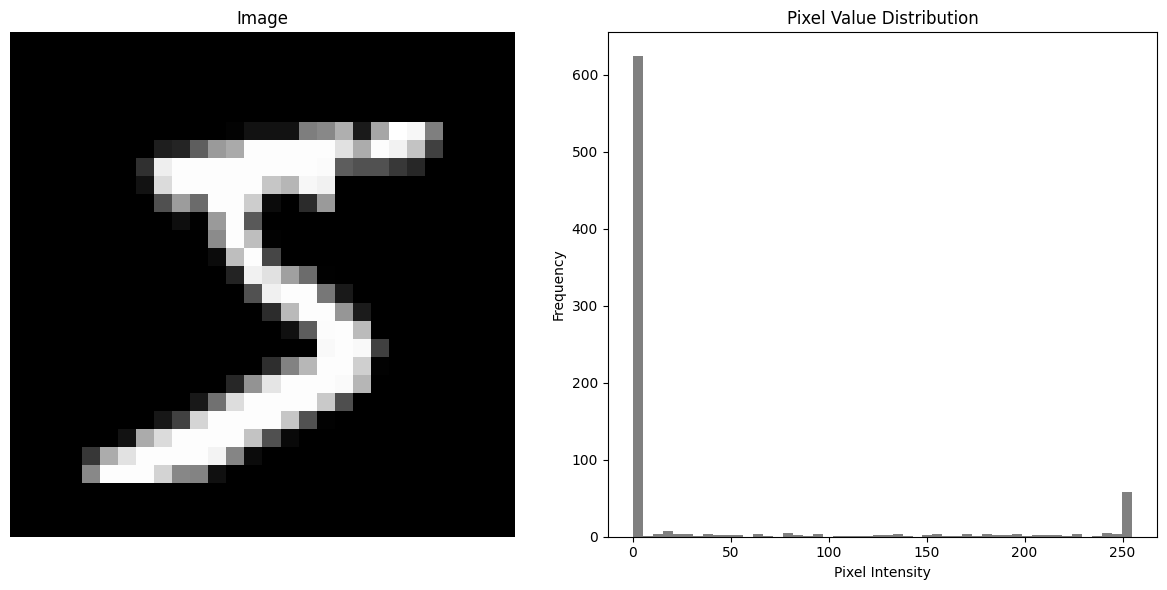
\includegraphics[width=0.75\textwidth]{Figures/Methods/MNIST_5_with_histogram.png}
    \caption{The first image in the MNIST training dataset; digit 5 and its pixel value distribution histogram scaled to 0-255 pixel intensity values.}
    \label{fig:mnist_5_histogram}
\end{figure}
As shown in Figure~\ref{fig:mnist_5_histogram}, the MNIST digit 5 is displayed alongside its pixel value distribution histogram where the pixel values range from 0 to 255. Figure~\ref{fig:mnist_0_histogram} shows the second image (zero) in the MNIST training dataset.

\begin{figure}[h]
    \centering
    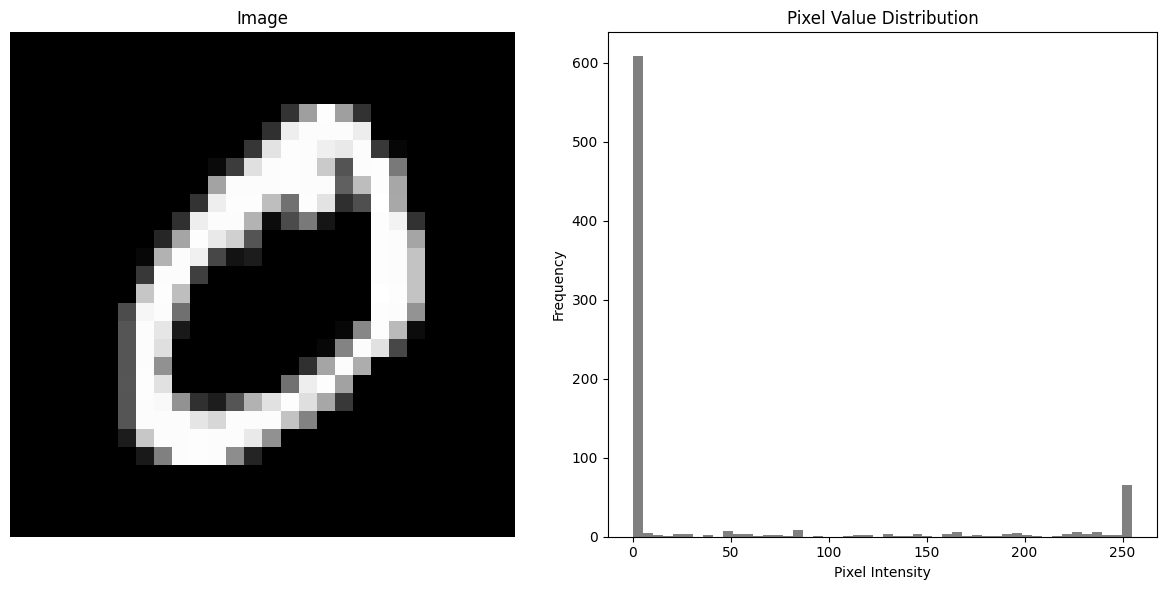
\includegraphics[width=0.75\textwidth]{Figures/Methods/MNIST_0_with_histogram.png}
    \caption{The second digit in the MNIST training dataset; digit 0 and its pixel value distribution histogram.}
    \label{fig:mnist_0_histogram}
\end{figure}

From the training labels dataset, it can be seen that by offsetting the magic number and the number of labels, represented by 4 bytes each, the following bytes represent the labels, that is, the first two labels are "05 and "00", matching figures \ref{fig:mnist_5_histogram} and \ref{fig:mnist_0_histogram}.

%%%%%%%%%%%%%%%%%%%%%%%%%%%%%%%%%%%%%
% CREATING THE NOISY PMNIST DATASET %
%%%%%%%%%%%%%%%%%%%%%%%%%%%%%%%%%%%%%

\subsubsection{Creating the "perturbed" PMNIST dataset}

To augment the research on image recognition robustness, we propose the creation of an enhanced training and testing dataset derived from the original MNIST dataset. This new dataset incorporates a variety of perturbations to the original images, aiming to simulate real-world conditions where image data may not be ideal. Specifically, we introduce noise to the images using 12 distinct functions, as described in Section \ref{methods:noise_perturbation}, designed to add perturbations, categorized as follows:

\begin{enumerate}
    \item \textbf{Pixel Intensity Adjustment:}
    \begin{itemize}
        \item Brightness
        \item Contrast
    \end{itemize}
    \item \textbf{Blurring:}
    \begin{itemize}
        \item Defocus Blur
        \item Motion Blur
        \item Zoom Blur
    \end{itemize}
    \item \textbf{Noise:}
    \begin{itemize}
        \item Gaussian Noise
        \item Impulse Noise
        \item Shot Noise
    \end{itemize}
    \item \textbf{Weather:}
    \begin{itemize}
        \item Fog
        \item Frost
        \item Snow
    \end{itemize}
    \item \textbf{Special Effects:}
    \begin{itemize}
        \item Pixelation
    \end{itemize}
\end{enumerate}

Each image in the original testing dataset undergoes a transformation by all perturbation methods, resulting in a companion image that retains the original label but exhibits the added noise or effect. The new dataset consist of the clean (original) and the noisy (perturbed) versions. 
%**TODO, describe new method storing perturbation and level in lower and upper nibbles.**
To distinguish and subsequent analysis, labels will be appended to denote the image type: "0xFF" for clean/original images and "01" for noisy/perturbed images. This dual dataset structure will enable comprehensive evaluation of machine learning models' performance in recognizing digits under varied noise regimes.
%, thereby enhancing the robustness of our image recognition pipeline.

% Applying noise

To generate our new dataset, we write to a binary file named perturbed-train-images-idx3-ubyte, where the first 16 bytes are:
\begin{verbatim}
0000 0803 0001 d4c0 0000 001c 0000 001c    
\end{verbatim}
Where 0001 d4c0 hex is 120000 decimal, the size of the new training dataset, twice the size of the original dataset.

We make a random selection of a perturbation type, and a perturbation level ranging from 0 to 9, and apply the perturbation to the image.

Figures \ref{fig:MNIST_4_clean_with_histogram} and \ref{fig:MNIST_4_noisy_with_histogram} show digit 4 with no noise and zoom blur level 8 applied.
\begin{figure}[h]
    \centering
    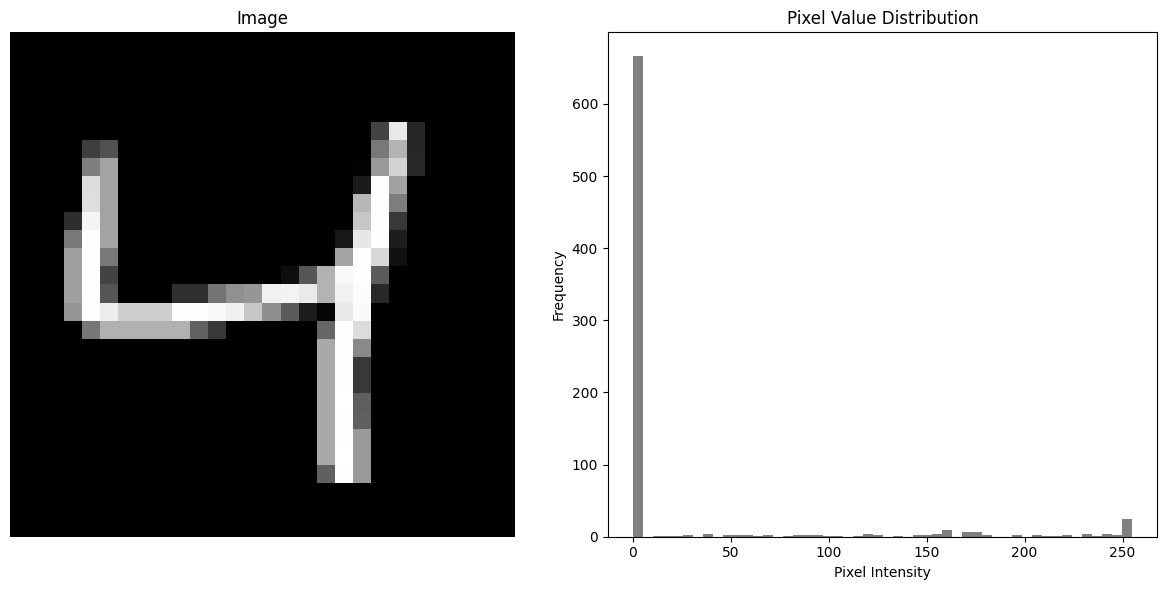
\includegraphics[width=0.75\textwidth]{Figures/Methods/MNIST_4_clean_with_histogram.png}
    \caption{MNIST digit 4 with no noise.}
    \label{fig:MNIST_4_clean_with_histogram}
\end{figure}

\begin{figure}[h]
    \centering
    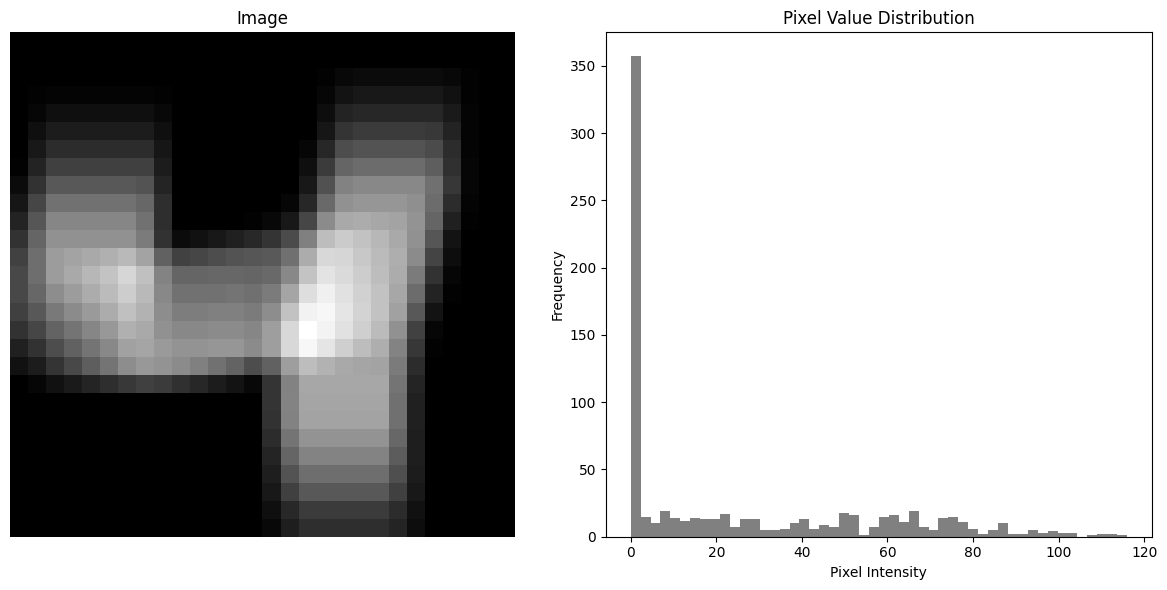
\includegraphics[width=0.75\textwidth]{Figures/Methods/MNIST_4_noisy_with_histogram.png}
    \caption{MNIST digit 4 with Zoom Blur level 8.}
    \label{fig:MNIST_4_noisy_with_histogram}
\end{figure}

% file to generate images is
% https://colab.research.google.com/drive/1s-KBSwUtT7tp280iLi8KgyHk4zThDnKD#scrollTo=OMq-a-wuKqR0
% MNIST-Dataset.ipynb

The process can be describe like so:

\begin{lstlisting}[caption={MNIST Perturbation Algorithm}, label={lst:mnist_perturbation_algorithm}]
Function createFiles():
    Open images.bin as binary write
    Open labels.bin as binary write
    Open perturbations.bin as binary write

Function saveImage(image, file):
    Write image to file

Function saveLabel(label, file):
    Write label to file as a single byte

Function savePerturbation(perturbationCode, file):
    Write perturbationCode to file as bytes

Function main():
    createFiles()
    For each image in MNIST:
        saveImage(originalImage, images.bin)
        saveLabel(0x00, labels.bin)
        savePerturbation(0xFFFF, perturbations.bin)
        
        perturbedImage = applyRandomPerturbation(originalImage)
        saveImage(perturbedImage, images.bin)
        saveLabel(0x01, labels.bin)
        perturbationCode = getPerturbationCode()
        savePerturbation(perturbationCode, perturbations.bin)

\end{lstlisting}

We apply the same process to training and testing datasets, and end up with 6 files as shown in Table \ref{table:mnist_perturbed_files_b}.

% \begin{table}[h]
% \centering
% \begin{tabular}{|l|l|r|r|}
% \hline
% \textbf{Type}             & \textbf{File Name}                          & \textbf{Size (B)} & \textbf{Count} \\ \hline
% Perturbed Training Images  & \texttt{perturbed-train-images-idx3-ubyte}    & TBA               & 120000 \\                            
% Perturbed Training Labels  & \texttt{perturbed-train-labels-idx1-ubyte}    & TBA               & 120000 \\                            
% Perturbation Training Levels  & \texttt{perturbation-train-levels-idx0-ubyte} & TBA               & 120000 \\
% Perturbed Testing Images   & \texttt{t20k-perturbed-images-idx3-ubyte}     & TBA               & 20000 \\                            
% Perturbed Testing Labels   & \texttt{t20k-perturbed-labels-idx1-ubyte}     & TBA               & 20000 \\  
% Perturbation Testing Levels   & \texttt{t20k-perturbation-levels-idx0-ubyte}     & TBA               & 20000 \\ \hline                 
% \end{tabular}
% \caption{Perturbed MNIST (PMNIST) Dataset Files, file sizes in bytes and image/label count}
% \label{table:mnist_perturbed_files_b}
% \end{table}

\begin{table}[h]
\centering
{\small
\begin{tabular}{|l|l|l|r|r|}
\hline
\textbf{ID} & \textbf{Type}                   & \textbf{File Name}                                   & \textbf{Size (M)} & \textbf{Count} \\ \hline
% 1 & Perturbed Training Images       & \texttt{perturbed-train-images-idx3-ubyte}    & TBA               & 7260000 \\
% 2 & Perturbed Training Labels       & \texttt{perturbed-train-labels-idx1-ubyte}    & TBA               & 7260000 \\
% 3 & Perturbation Training Levels    & \texttt{perturbation-train-levels-idx0-ubyte} & TBA               & 7260000 \\
1 & Perturbed Testing Images        & \texttt{t1210k-perturbed-images-idx3-ubyte}     & 905M               & 1210000 \\
2 & Perturbed Testing Labels        & \texttt{t1210k-perturbed-labels-idx1-ubyte}     & 1.2M               & 1210000 \\
3 & Perturbation Testing Levels     & \texttt{t1210k-perturbation-levels-idx0-ubyte}  & 1.2M               & 1210000 \\ \hline
\end{tabular}
} % End of \small
\caption{Perturbed MNIST (PMNIST) Dataset Files, file sizes in bytes and image/label count}
\label{table:mnist_perturbed_files_b}
\end{table}

Where the additional files are perturbation-train-levels-idx0-ubyte and t20k-perturbation-levels-idx0-ubyte that contain the perturbation types and levels, stored contiguously in one byte values. As per the algorithm listed in Listing \ref{lst:mnist_perturbation_algorithm}, We start by opening the binary files. We then iterate over every image in the MNIST dataset. We apply a random perturbation and perturbation level to the image, writing the original and perturbed image to the new PMNIST dataset (ID 1). We write the image label twice (ID 2), once with value 0 indicating the image is noise-free, and once with value 1 indicating the image is perturbed, aligning with the saved images and finally we write the perturbation key and level (ID 3). We repeat the steps for the testing dataset, obtaining 3 additional files (IDs 4, 5 and 6).

% TODO HANDWRITTEN DIGITS

% TODO HANDWRITTEN CHARACTERS

% TODO MNISTified CIFAR-10

% SELF-DRIVING DATASETS
% REGRESSION
% REGRESSION SEGMENTED
% REGRESSION SEGMENTED WITH FIDUCIALS
% CLASSIFICATION SEGMENTED
% CLASSIFICATION SEGMENTED 3 bin unbalanced
% CLASSIFICATION SEGMENTED 3 bin balanced
% CLASSIFICATION SEGMENTED 5 bin unbalanced
% CLASSIFICATION SEGMENTED 5 bin balanced
% CLASSIFICATION SEGMENTED 15 bin unbalanced
% CLASSIFICATION SEGMENTED 15 bin balanced
% NB VLMs use 3 bin balanced/unbalanced.

%%%%%%%%%%%%%%%%%%
% MNIST VARIANTS %
%%%%%%%%%%%%%%%%%%

\subsection{MNIST Variants}
% TODO This figure is REPEATED in results, so one has to go, probably this one, then refer to results, or vice-versa
\begin{figure}[h]
\centering
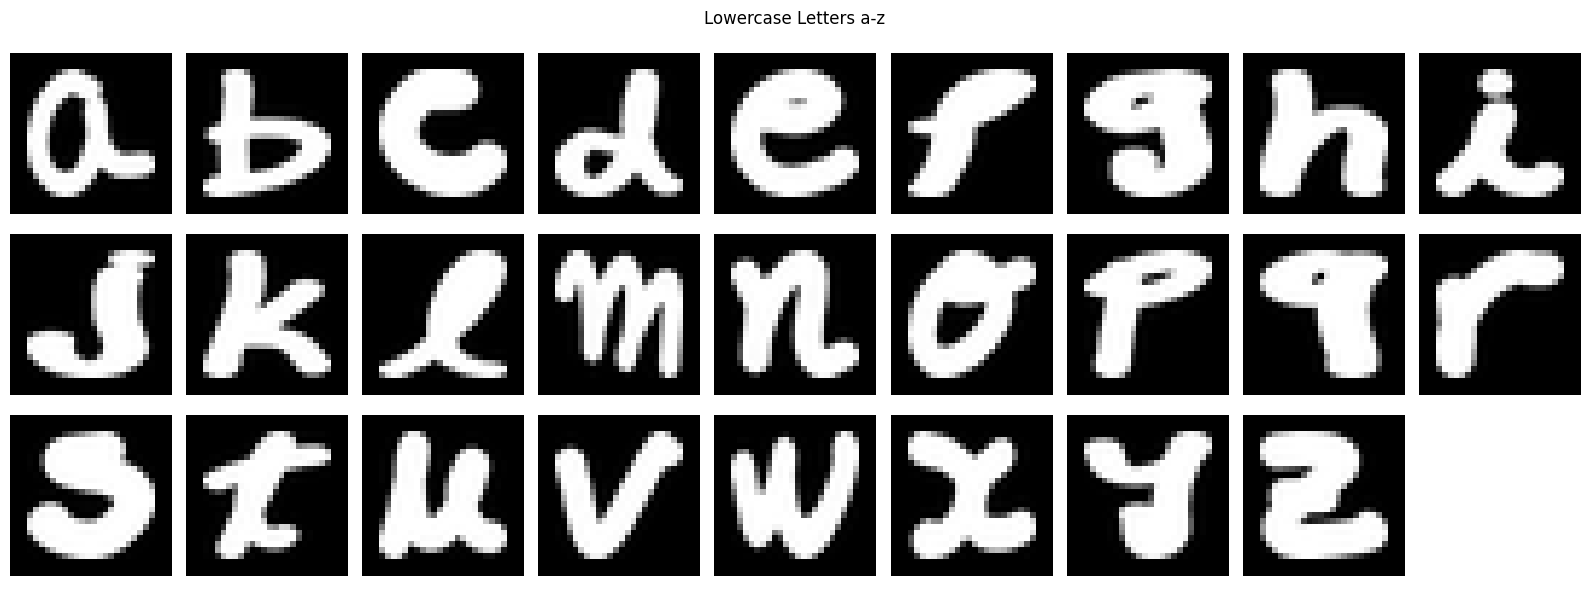
\includegraphics[width=0.99\textwidth]{Figures/Results/HandwrittenCharacters/mnistified-a-z.png}
\caption{Example of the MNISTified English handwritten lower case alphabetical characters.}
\label{fig:mnistified-a-z-methods}
\end{figure}

\textbf{MNISTified English Handwritten Characters - Digits and Alphabetical Characters} dataset \cite{deCampos09} subject a CNN trained on MNIST to broader character sets. The base dataset contains 3,410 images of handwritten English characters across 62 classes: digits 0-9, uppercase A-Z, and lowercase a-z as shown in Figure \ref{fig:mnistified-a-z-methods}, with 55 images per class.
Images were preprocessed to match MNIST format: inverted to white characters on black backgrounds, resized to 28×28 pixels, and trimmed to remove excess margins. This preprocessing enables direct application of MNIST-trained models to character data.
The datasets test model performance across distribution shifts. The digits subset provides near-distribution evaluation, containing the same character types as MNIST training data. The alphabetical subset introduces varying degrees of out-of-distribution challenge, from characters visually similar to digits (Z resembles 2, upper case B resembles 8, lowercase b resembles 6) to completely dissimilar characters with no digit-like features.
This progression from in-distribution digits to out-of-distribution alphabetical characters allows systematic evaluation of how distance-based safety measures respond to increasing distribution shift.

\textbf{MNISTified CIFAR-10} converts CIFAR-10 color images to 28×28 grayscale format, matching MNIST dimensions.

%%%%%%%%%%%%%%%%%%%%%%%%%
% SELF-DRIVING DATASETS %
%%%%%%%%%%%%%%%%%%%%%%%%%

\subsection{Self-Driving Datasets}

\begin{figure}[h]
\centering
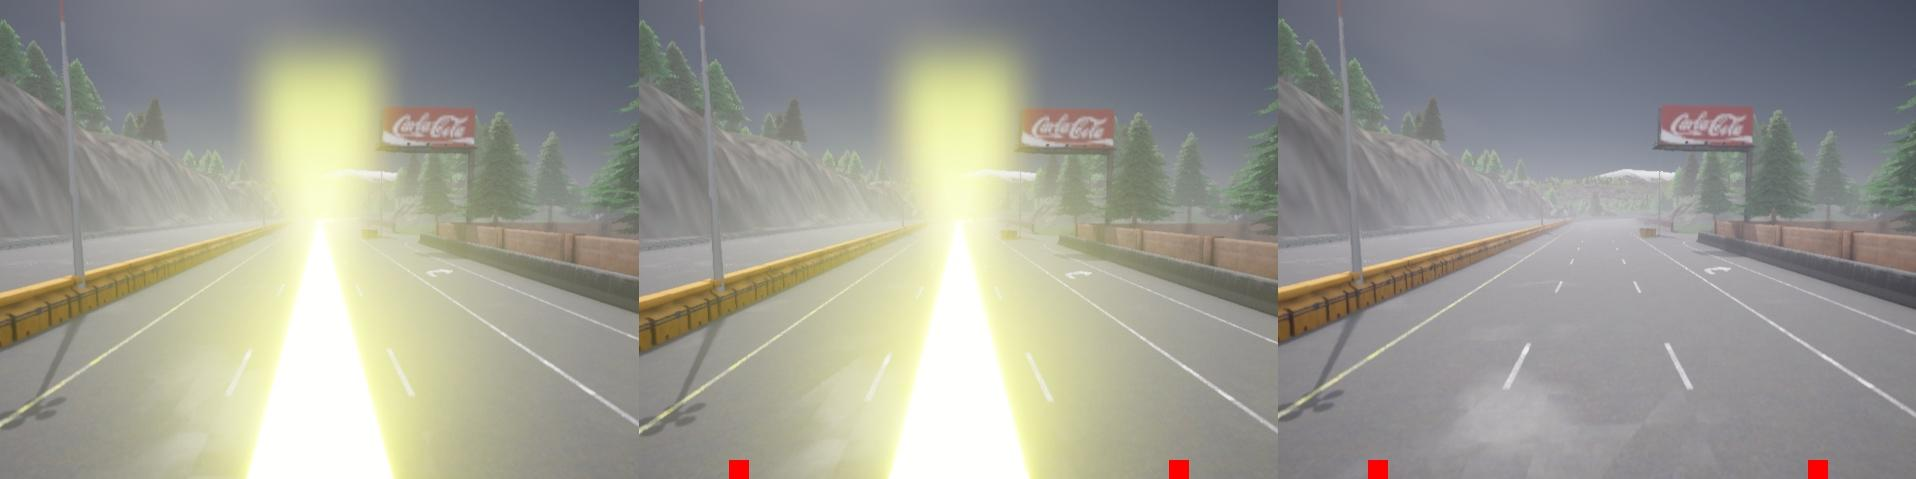
\includegraphics[width=0.99\textwidth]{Figures/Methods/carla_dataset_seg_segfid_fid.jpg}
\caption{Images captured with a CARLA simulated vehicle front facing camera, from left to right, with road segmentation, road segmentation and fiducial markers and fiducial markers only, where the most commonly used image type used in this study were images with road segmentation only (left).}
\label{fig:carla_dataset_seg_segfid_fid}
\end{figure}

We capture datasets (with images as displayed in Figure \ref{fig:carla_dataset_seg_segfid_fid}) using the process described in subsection \ref{methods:carla_gen_train_datasets}. Datasets may have continuous or quantized steering angle labels, additionally the images could be raw, contain lane segmentation, contain lane segmentation and fiducial markers.
 
Lane segmentation for autonomous driving has evolved from classical image processing to deep learning-based, pixel-wise semantic segmentation, often using UNet-like architectures. However, to meet real-time demands and handle occlusions, recent methods reframe the task as a row-based classification problem using global features, achieving significantly higher speeds \cite{qin2020ultra}. Conversely, fiducial markers like AprilTag provide robust 6-DOF pose estimation for robotics by introducing engineered, high-contrast patterns into the environment, simplifying perception into a problem of detecting known landmarks and solving for camera pose \cite{olson2011tags}.

Lane segmentation is a staple in self-driving, we create lane segmentation by using a specific feature of the CARLA simulator - connecting waypoints with markers, although lane segmentation itself does exist as a standalone feature in CARLA.

%%%%%%%%%%%%%%%%%%%%%%%%%%%%%%%%%%%%%%%
% SELF-DRIVING DATASETS - REGRESSSION %
%%%%%%%%%%%%%%%%%%%%%%%%%%%%%%%%%%%%%%%

\subsubsection{Self-Driving Datasets - Regression}

Three regression dataset variants predict continuous steering angle values from camera images:

\textbf{Vanilla} uses raw camera images as input with continuous steering angle targets.

\textbf{Segmented} - Vanilla plus lane segmentation.

\textbf{Segmented with Fiducials} - segmented plus fiducial makers.

%%%%%%%%%%%%%%%%%%%%%%%%%%%%%%%%%%%%%%%
% SELF-DRIVING DATASETS - REGRESSSION %
%%%%%%%%%%%%%%%%%%%%%%%%%%%%%%%%%%%%%%%

\subsubsection{Self-Driving Datasets - Classification}

Steering angles are quantized into discrete bins for classification tasks. Three binning schemes are implemented:

\begin{align*}
\text{3-bin:} &\quad [-0.065, 0.0, 0.065] \\
\text{5-bin:} &\quad [-0.065, -0.015, 0.0, 0.015, 0.065] \\
\text{15-bin:} &\quad [-0.065, -0.055, -0.045, -0.035, -0.025, \\
&\quad\quad -0.015, -0.005, 0.0, 0.005, 0.015, \\
&\quad\quad 0.025, 0.035, 0.045, 0.055, 0.065]
\end{align*}

Each binning scheme generates two dataset variants:

\textbf{Unbalanced} datasets preserve natural steering angle distributions where straight driving dominates.

\textbf{Balanced} datasets have randomly duplicated minority class images such that all classes contain equal numbers of training examples.

Vision Language Models use 3-bin balanced and unbalanced variants.

%%%%%%%%%%%%%%%%%%%%%%%%%%%%%%%%
% NEURAL NETWORK ARCHITECTURES %
%%%%%%%%%%%%%%%%%%%%%%%%%%%%%%%%

\subsection{CNN, ViT and VLM Architectures}
\label{methods:neural_architectures}

\textbf{Convolutional Neural Networks (CNNs)} process images through hierarchical feature extraction \cite{lecun1998gradient}. Convolutional layers apply learnable filters across input images to generate feature maps detecting edges, textures, and objects. ReLU activation introduces non-linearity. Pooling layers downsample feature maps for computational efficiency and translation invariance. Fully connected layers perform final classification using extracted high-level features.

\textbf{Vision Transformers (ViTs)} treat images as sequences of fixed-size patches \cite{dosovitskiy2021image}. Each patch is flattened and embedded into vector space with positional encodings preserving spatial relationships. A classification token aggregates global image representation. Multi-head self-attention mechanisms enable each patch to attend to all others, capturing long-range dependencies. Feed-forward networks process attention outputs before final classification.

\textbf{Vision-Language Models (VLMs)} integrate visual and textual processing through specialized architectures. Qwen-VL combines a ViT visual encoder with the Qwen LLM backbone \cite{bai2023qwen}. A position-aware cross-attention adapter compresses visual features from 1024+ tokens to 256 fixed-length representations for efficient LLM processing. DeepSeek-VL employs hybrid vision encoding: SigLIP-L processes low-resolution semantic features while SAM-B captures high-resolution details \cite{zeng2024deepseek}. A two-layer MLP adapter fuses these representations into 576 visual tokens for the DeepSeek-LLM backbone.

%%%%%%%%%%%%%%%%%%%%%%%%%%%%%%%%%%%
% NETWORK TRAINING & EVALUATION   %
%%%%%%%%%%%%%%%%%%%%%%%%%%%%%%%%%%%
\section{Network Training and Evaluation}
\label{methods:training}

\subsection{CNN}
Images undergo three preprocessing steps before CNN input. Vertical cropping removes sky and hood regions, retaining pixels from y-coordinate 210 to 480. Spatial downsampling resizes cropped images to 200×66 pixels using bilinear interpolation. Color space conversion transforms RGB to YUV \cite{lecun2004dave, bojarski2016end} N.B. Although there is a biological motivation to transform RGB to YUV \cite{podpora2014yuv}. In the RGB scheme, each pixel is represented by three channel intensities of red, green and blue. In YUV, also referred to as YCbCr (\cite{maller2020}) space, each pixel is represented by Y (luma), U (Cb - luminance value subtracted from red channel) and V (Cr - luminance value subtracted from red channel). It is a "lossy" process which degrades the data, and originally developed for colour to black and white television backward compatibility. Moving the image from RGB to YUV space has been demonstrated to give "better subjective image quality than the RGB color space", being better for computer vision "implementations than RGB due to the perceptual similarities to the human vision" (\cite{podpora2014yuv}). No data augmentation is applied. 

The CNN implements the NVIDIA architecture from Bojarski et al. (2016) \cite{bojarski2016end} with standard regression and modifications for classification outputs. Five convolutional layers use ELU activation with kernel sizes [5,5,5,3,3] and strides [2,2,2,1,1]. Channel progression follows [24,32,48,64,64]. Four fully connected layers with dimensions [1152,100,50,10] precede the output layer. Dropout with probability 0.1 follows each layer. Input normalization divides pixel values by 255.

Training uses an 80/20 random train-validation split with shuffled indices. Adam optimizer applies learning rate 1e-5 with default momentum parameters. Cross-entropy loss trains classification variants; mean squared error trains regression variants. Batch size is 64 samples. Training runs for maximum 100 epochs with early stopping monitoring validation loss. Early stopping triggers after 6 epochs without improvement, restoring the best model state. Training executes on NVIDIA GPU with CUDA acceleration. Best-performing models save as PyTorch state dictionaries including model weights, optimizer state, epoch number, and final loss values.

\subsection{ViT from scratch}
\label{methods:vit_from_scratch}
Vision Transformers train from scratch using patch-based image tokenization. Images are divided into non-overlapping patches of size 8×8 pixels for CIFAR-10 and 4×4 pixels for MNIST. Each patch is flattened and linearly projected to embedding dimension 64. Positional embeddings are added to patch embeddings before input to the transformer encoder.

The transformer architecture uses 6 encoder layers with 4 attention heads per layer. Each encoder layer contains multi-head self-attention followed by a feed-forward network with expansion factor 2. Dropout probability is 0.1 for all layers. Layer normalization applies before attention and feed-forward blocks following the pre-norm configuration.

Training uses Adam optimizer with peak learning rate 5e-4 and 10-epoch linear warmup. Batch size is 128 samples. Training runs for 5000 epochs without early stopping. RandAugment data augmentation applies during training with default parameters. Training executes on GPU when available with automatic fallback to CPU. Model checkpoints save based on configurable frequency, with final models stored as complete state dictionaries.

\subsection{Pre-trained ViT Fine-tuning}

Pre-trained Vision Transformer fine-tuning adapts Google's ViT-base-patch16-224 (\cite{google2021vitbasepatch16224}) weights for both regression and classification tasks. Models initialize with ImageNet weights. Classification heads modify original 1000-class outputs to task-specific dimensions: single output for regression, N outputs for N-class classification.
Image preprocessing standardizes inputs to 224×224 pixel resolution for both variants. Dataset creation extracts steering angle labels from CARLA image metadata. Images convert to RGB format before processing. Dataset splits use 80/20 random train-validation division.
Training applies identical configurations across task types. Batch size sets to 16 samples per device for training and evaluation. Learning rate uses 2e-5 with 30 training epochs. Evaluation runs per epoch with matching save frequency.
Loss functions differ by task: mean squared error for regression variants, cross-entropy loss for classification variants. Regression evaluation computes MAE and MSE. Classification evaluation computes accuracy from predicted classes. Best model selection uses task-appropriate metrics: MAE minimization for regression, accuracy maximization for classification.
Model checkpointing saves every 500 steps with maximum three checkpoints retained. Training logs save to timestamped directories with automatic visualization. Final models save as complete directories containing weights, configuration, and preprocessing parameters.

%%%%%%%%%%%%%%%%%%%%%%%%%%%%%%%%%%%%%%%%%%%%
% VISION-LANGUAGE MODEL ZERO-SHOT LEARNING %
%%%%%%%%%%%%%%%%%%%%%%%%%%%%%%%%%%%%%%%%%%%%

\subsection{Zero-Shot Vision Language Model Evaluation}
To establish a performance baseline of VLM scene understanding, the meta-llama/Llama-3.2-11B-Vision-Instruct (\cite{meta2024llama3vision} model was evaluated on the CIFAR-10 dataset in a zero-shot setting. This assessment measured the model's intrinsic visual understanding capabilities without any task-specific training or fine-tuning. The evaluation protocol involved presenting the model with CIFAR-10 images at three distinct input resolutions: standard 32x32, 720x720, and 1440x1440 pixels. 

%%%%%%%%%%%%%%%%%%%%%%%%%%%%%%%%%%%%%
% VISION-LANGUAGE MODEL FINE-TUNING %
%%%%%%%%%%%%%%%%%%%%%%%%%%%%%%%%%%%%%

\subsection{Vision-Language Model Fine-Tuning}
Vision-language model fine-tuning adapts Qwen2-VL-2B-Instruct \cite{bai2023qwen} for steering decision tasks using supervised fine-tuning with conversational data. The base model initializes with pre-trained multimodal weights supporting both vision and language understanding.

Dataset preparation extracts steering angles from CARLA image filenames and maps binned  values to verbal directional commands. Three steering bins define the classification space: 0.0000 maps to "Straight", -0.0650 maps to "Left", and 0.0650 maps to "Right". Each sample pairs CARLA simulator images with a fixed query prompt "What direction the vehicle should be steering?" and corresponding directional labels.

Training data structures as three-role conversations following chat template formatting. System messages define the model as a steering specialist constrained to output only directional commands. User messages combine CARLA images with steering queries. Assistant messages provide single-word directional responses matching the three-class label space.

Fine-tuning applies QLoRA \cite{dettmers2023qlora} parameter-efficient training targeting query and value projection layers. LoRA \cite{hu2021lora} configuration uses rank 8 with alpha 16 and 5\% dropout. Training runs for 3 epochs with batch size 4 per device and gradient accumulation over 8 steps. Learning rate sets to 2e-4 with constant scheduling and 3\% warmup ratio.
Loss computation applies standard causal language modeling with special handling for vision tokens. Image token embeddings exclude from loss calculation to focus learning on text generation. Gradient checkpointing enables training within memory constraints while maintaining bfloat16 precision throughout.

Model checkpointing saves every 20 steps with evaluation-based selection using validation loss minimization. Final models save as complete directories containing adapted weights, tokenizer configuration, and image processor settings.

\section{Network Evaluation}

Network evaluation can be categorized in two cases, where the CARLA simulator is required, and where the CARLA simulator is not required. In the latter case, the dataset, be it for self-driving regression or classification, or CIFAR-10, MNIST and MNISTified datasets, can be accessed in a single inference loop, are not subject to the contraints described next.
Network evaluation for realtime self-driving operates under constraints imposed by CARLA simulator compatibility requirements. CARLA 0.9.13 requires Python 3.6.9 for API wrapper functionality, while the transformers libraries requires Python 3.11.0 or greater. Two different evaluation schemes addressed in the following subsections are used to address the issue.

\subsection{CNN Single-Environment Evaluation}

CNN evaluation (no transformers model required) runs entirely within Python 3.6.9 environment. CARLA simulation and CNN inference execute in the same environment space, enabling direct model integration within the simulation loop.

\subsection{ViT/VLM Dual-Environment Evaluation}
\begin{figure}[h]
\centering
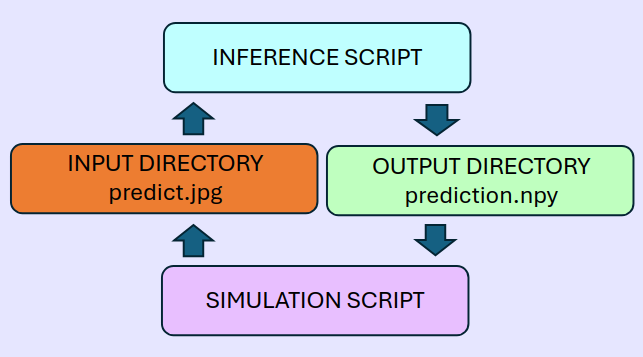
\includegraphics[width=0.50\textwidth]{Figures/Methods/LocalVLMInference.png}
\caption{Local ViT/VLM inference workflow, where a simulation script generates an output image predict.jpg taken from vehicle's front facing camera and the inference script generates a softmax output predict.npy that the simulation script collects to then extract the steering angle that should be applied to the simulated vehicle.}
\label{fig:LocalVLMInference}
\end{figure}

As previously mentioned, ViT (as well as VLM) evaluation requires separate Python environments. CARLA simulation is controlled in a Python 3.6.9 environment while ViT inference runs in a Python 3.11.0 environment. Inter-process communication bridges the two environments, transferring image data from simulation to inference process and returning steering predictions. This architecture introduces additional latency through disk-based communication. Images write to disk from CARLA simulation and read from disk by ViT inference process. Predictions write to disk by ViT inference as plain text files containing single float steering angles for regression tasks or as pickle files containing softmax outputs for classification tasks. CARLA simulation subsequently reads prediction files from disk. The simulation process takes care of reading the prediction file, then deleting the prediction file and writing an image file to disk e.g. predict.jpg . The inference process takes care of reading the image, then deleting the image and writing the inference file to disk e.g. prediction.npy. The flow (excluding file deletions) is shown in Figure \ref{fig:LocalVLMInference}.

\begin{figure}[h]
\centering
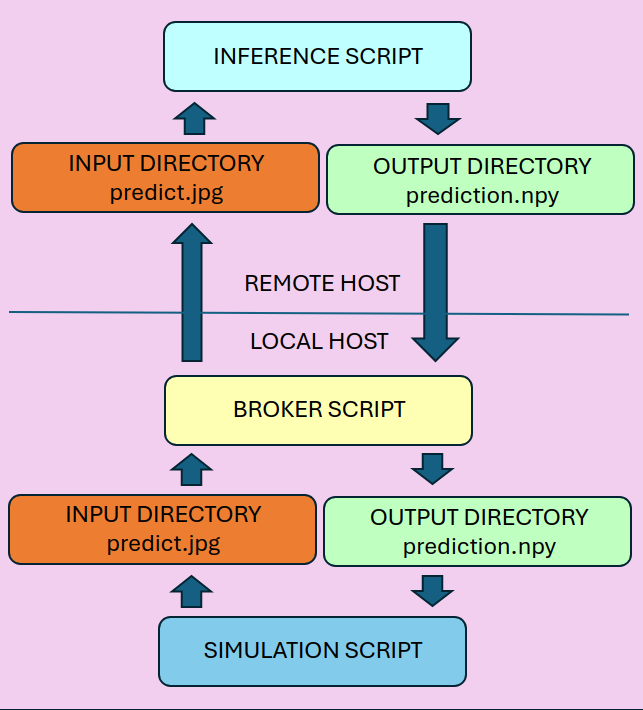
\includegraphics[width=0.50\textwidth]{Figures/Methods/RemoteVLMInference.png}
\caption{Remote VLM inference workflow, where a simulation script generates an output image predict.jpg taken from vehicle's front facing camera, the broker script transfers to the remote host, the inference script generates a softmax output predict.npy that the broker transfers to local host, finally simulation script collects to then extract the steering angle that should be applied to the simulated vehicle.}
\label{fig:RemoteVLMInference}
\end{figure}

% \begin{verbatim}                                    
% +-------------------------------------+
% |           INFERENCE SCRIPT          |
% +-----------------------------+-------+
%          ^                    |       
%          |                    v       
% +-----------------+ +------------------+
% | INPUT DIRECTORY | | OUTPUT DIRECTORY |
% | predict.jpg     | | prediction.npy   |
% +-----------------+ +--------+---------+
%          ^                    |       
%          |                    v       
% +-------------------------------------+
% |         SIMULATION SCRIPT           |     
% +-------------------------------------+
% \end{verbatim}


\subsection{VLM Remote Evaluation}

VLM evaluation addresses memory constraints through remote inference deployment. The local workstation does not have enough GPU memory to run Qwen2-VL model inference at the same time, so the inference is run on the HPC cluster. Image and prediction file exchange occurs in the same way as with the local dual-environment, with the addition of a broker process that takes care to transfer files from local to remote filesystems and back gain, while also dealing with file deletions. The flow is described in Figure \ref{fig:RemoteVLMInference}. The process is described in greater detail in experiment 290. 

% \begin{verbatim}
% +-------------------------------------+
% |           INFERENCE SCRIPT          |
% +-----------------------------+-------+
%          ^                    |       
%          |                    v       
% +---------+-------+ +------------------+
% | INPUT DIRECTORY | | OUTPUT DIRECTORY |
% | predict.jpg     | | prediction.npy   |
% +-----------------+ +--------+---------+
%          ^   REMOTE HOST     |       
% ---------+--------------------+--------
%          |   LOCAL HOST      |       
% +---------+--------------------+-------+
% |           BROKER SCRIPT             |
% +--------+--------------------+-------+
%          |                    |       
%          |                    v       
% +---------+--------+ +------------------+
% | INPUT DIRECTORY | | OUTPUT DIRECTORY |
% | predict.jpg     | | prediction.npy   |
% +-----------------+ +--------+---------+
%          ^                    |       
%          |                    v       
% +-------------------------------------+
% |         SIMULATION SCRIPT           |
% +-------------------------------------+
% \end{verbatim}   

% \ref{app_res:290}.

%%%%%%%%%%%%%%%%%%%%%%%%%%%%%%%%
% SOFTMAX CLUSTERING ALGORITHM %
%%%%%%%%%%%%%%%%%%%%%%%%%%%%%%%%

\section{Softmax Clustering for Uncertainty Quantification}
\label{methods:clustering}

\sloppy

We consider a neural network output vector $\mathbf{p} = (p_1, p_2, \dots, p_K)$ where $\sum p_i = 1$, representing a probability distribution obtained by normalizing the logit vector $\mathbf{z} = (z_1, z_2, \dots, z_K)$ through the softmax function, $p_i = \text{softmax}(z_i) = e^{z_i} / \sum_{j=1}^{K} e^{z_j}$. For example, given $\mathbf{p} = [0.01, 0.01, 0.01, 0.01, 0.9, 0.01, 0.01, 0.01, 0.01, 0.01]$, the predicted class is '4', corresponding to the highest value at index five, reflecting the confidence of the prediction for each class from '0' to '9'. The logits, representing log-likelihoods of class memberships, are related to probabilities by $z_i = \log (p_i / (1 - p_i))$ where $z_i$ is the logit for class $i$, and $p_i$ is the probability of the input belonging to class $i$.
%\cite{goodfellow2016deep,bishop2006pattern}.

We store the predictions for MNIST and CIFAR-10 datasets in a matrix $\mathbf{M} \in \mathbb{R}^{n \times 12}$, where $n$ is the number of predictions, the first ten columns are the softmax probabilities, column 11 is the true class and column 12 is the predicted class.
To obtain cluster centroids $\mathbf{C} \in \mathbb{R}^{10 \times 10}$ we calculate the mean of all correct predictions from the training datasets with Algorithm \ref{alg:k-means-centroid-init}. To calculate the softmax distance threshold we use all incorrect predictions with Algorithm \ref{alg:min_distance}.

\begin{algorithm}
\caption{K-Means Centroid Initialisation from Softmax Outputs}
\label{alg:k-means-centroid-init} 
\begin{algorithmic}[1]
\Require{$correct\_preds$: array of shape $(n, 12)$, where $n$ is the number of correct predictions}
\Ensure{$centroids$: array of shape $(10, 10)$, initialised centroids for each digit class}

\State $probs\_dist \gets corrects\_preds[:, :10]$ \Comment{Extract probability distribution for each digit}
\State $centroids \gets \text{zeros}((10, 10))$ \Comment{Initialise centroids array}

\For{$digit \gets 0$ to $9$}
\State $indices \gets \text{where}(\text{argmax}(probs\_dist, \text{axis}=1) == digit)[0]$ \Comment{Find indices of rows where digit has highest probability}
\State $centroid \gets \text{mean}(probs\_dist[indices], \text{axis}=0)$ \Comment{Compute mean probability distribution for selected rows}
\State $centroids[digit] \gets centroid$ \Comment{Assign centroid to corresponding row in centroids array}
\EndFor

\State \textbf{return} $centroids$
\end{algorithmic}
\end{algorithm}

%%%%%%%%%%%%%%%%%%%%%%%%%%%%%
% GEOMETRIC CHARACTERISTICS %
%%%%%%%%%%%%%%%%%%%%%%%%%%%%%

\textbf{Geometric Characteristics of Probability-Constrained Cluster Spaces}: Cluster centroids produced by  softmax layer outputs adhere to valid probability distributions. This requires each coordinate \( c_i \) to satisfy \( 0 \leq c_i \leq 1 \) and the sum \( \sum_{i=1}^n c_i = 1 \), confining the centroids to the vertices and interior of the standard \((n-1)\)-dimensional simplex. For two such centroids \( \mathbf{c}_1 \) and \( \mathbf{c}_2 \) within the \( n \)-dimensional unit hypercube under these constraints, the Euclidean distance between centroids \( \mathbf{c}_1, \mathbf{c}_2 \in [0,1]^n \) is \( d(\mathbf{c}_1, \mathbf{c}_2) = \sqrt{\sum_{i=1}^{n}\left(c_{1i} - c_{2i}\right)^2} \). When enforcing probabilistic constraints via softmax normalization, the maximum achievable distance between centroids remains bounded by \(\sqrt{2}\), independent of the dimensionality \( n \).

\begin{algorithm}
\caption{Find Minimum Softmax Distances to Centroids for Incorrectly Predicted Digits (Threshold)}
\label{alg:min_distance} 
\begin{algorithmic}[1]
\Procedure{FindMinDistances}{$data$}
    \State $labels \gets [0, 1, 2, 3, 4, 5, 6, 7, 8, 9]$
    \State $thresh \gets \text{empty array of shape } (10, 2)$
    \For{$i \gets 0 \text{ to } 9$}
        \State $label \gets labels[i]$
        \State $min\_dist \gets \min(data[data[:, 1] == label, 0])$
        \State $thresh[i, 0] \gets min\_dist$
        \State $thresh[i, 1] \gets label$
    \EndFor
    \State \textbf{return} $thresh$
\EndProcedure
\end{algorithmic}
\end{algorithm}

\textbf{Cluster Density}: Quantifying cluster density in high-dimensional softmax spaces provides insight into the confidence of neural network predictions. The density of a cluster in an $n$-dimensional space is quantified using the following equations:
\begin{equation}
\rho_k = \frac{N_k}{V_n(r_k)}, \quad V_n(r_k) = \frac{\pi^{n/2}}{\Gamma\left(\frac{n}{2} + 1\right)} r_k^n, \quad N_k = \sum_{i=1}^n \mathbf{1}(\|\mathbf{x}_i - \mathbf{c}\| \leq r_k) \label{eq:density_volume_count}
\end{equation}

\noindent where \(\rho_k\) is the cluster density for radius scaling factor \(k\) \cite{ester1996density}, \(N_k\) is the number of points within radius \(r_k\), \(V_n(r_k)\) is the volume of the \(n\)-dimensional hypersphere with radius \(r_k\) \cite{Conway1998}, \(r_k = k \cdot r\) is the scaled radius, \(k\) is the scaling factor, \(r\) is the base radius, \(n\) is the number of dimensions, \(\pi\) is the mathematical constant, \(\Gamma\) is the gamma function, \(\mathbf{1}\) is the indicator function, \(\mathbf{x}_i\) is the \(i\)-th point’s coordinates, \(\mathbf{c}\) is the cluster centroid, and \(\|\cdot\|\) is the Euclidean norm, measuring the distance between points \cite{Duda2000}. These enable evaluation of cluster compactness at varying radii \cite{Hastie2009}.

The volume $V_{shell}$ of a shell between inner and outer radii $r_1, r_2$  is given by:

\begin{equation}
V_{\text{shell}}(n, r_1, r_2) = \frac{\pi^{n/2}}{\Gamma(n/2 + 1)} \cdot \left( r_2^n - r_1^n \right)
\end{equation}

The number of points $N_{shell}$ in a shell is given by $ N_{shell}(r_1,r_2) = N_{r_2} - N_{r_1} $, where $N_{r_2}$ is the number of points within a hypersphere of radius $r_2$ and $N_{r_1}$ is the number of points within hypersphere of radius $r_1$, where both hyperspheres are concentric and $r_2 > r_1$.

In n-dimensional spaces, hypersphere shells demonstrate volume distribution patterns that differ significantly from low-dimensional intuition. For n > 5, the volume concentrates predominantly in outer shells, while exponentially decreasing toward the center. The ratio between consecutive shell volumes increases with dimension, creating a steep volume gradient. This concentration effect stems from the $r^n$ term in the above volume formula. This affects nearest-neighbor calculations and creates challenges for clustering algorithms with most points existing near the hypersphere's surface rather than distributed throughout its volume. To handle this issue, in our approach thresholds will be calculated w.r.t. the true and predicted classes in the training set.

%%%%%%%%%%%%%%%%%%%%%%%%%%%%%%%%%%%%%%%
% REGRESSION-TO-CLASSIFICATION TRANSFORM %
%%%%%%%%%%%%%%%%%%%%%%%%%%%%%%%%%%%%%%%
\section{Regression-to-Classification Transformation}
\label{methods:regression_classification}

To apply the method described in Section \ref{methods:clustering} to the self-driving steering-angle prediction problem, it is necessary to transform neural network regressors as seen in end-to-end learning approaches for autonomous driving (\cite{lecun2004dave,bojarski2016end}), into classifiers. The output layer was modified from one neuron producing a single continuous value to $N$ neurons corresponding to $N$ discrete bins classes. The final linear transformation changed from a mapping to $\mathbb{R}^1$ to a mapping to $\mathbb{R}^N$, where $N$ represents the number of steering angle bins (3, 5, or 15). 

The problem of selecting the number of bins when discretising continuous variables has been studied in the statistical literature on histogram construction. Classical approaches include Sturges’ rule (\cite{sturges1926}), Scott’s rule (\cite{scott1979}), and the Freedman–Diaconis rule (\cite{freedman1981}), while more recent work has proposed Bayesian and penalised-likelihood methods (\cite{knuth2006,birge2006}). These methods show that the optimal binning depends on sample size, data spread, and the intended task. The choice of bin numbers was determined empirically in this study, with 3 and 5 bins found to provide the best performance for steering classification, Sturge's, Scott's and Freedman-Diaconis suggest 16, 52 and 67 bins respectively, for 28k examples which is the typically size of the training dataset for self-driving.

The regression model outputs a single value interpreted directly as the predicted steering angle. The classification model outputs $N$ logits passed through softmax activation to produce binned steering angle class probabilities, where each class represents a steering angle. The number of bins must always be odd such that the middle bin corresponds to zero degree (straight) steering.

Loss functions changed from Mean Squared Error (MSE) for regression to Cross-Entropy Loss for classification. Evaluation metrics changed from Mean Absolute Error (MAE) to classification accuracy, calculated as the percentage of images where the predicted class matches the true class. Training procedures remained otherwise identical, including learning rates, batch sizes, and early stopping criteria (\cite{goodfellow2016deep}).




%%%%%%%%%%%%%%%%%%%%%
% VLM/MLLM METHODS %
%%%%%%%%%%%%%%%%%%%%%

% Last minute 2025.08.31 addition:
% See this survey:% https://www.sciencedirect.com/science/article/pii/S2949855424000613#sec2
% Section related work provides some good hooks into how VLMs evolved in
% scene understanding, to help robotics
% # 2. Related work and 2.2. Multimodal task planning with LLMs
% note "to foster a more holistic and nuanced AI-driven analysis" suggests
% written by LLM. LLMs writing about themselves
% Cited articles 29 through 43 seem like good candidates for lit survey

\section{Vision Language Model Implementation}
\label{methods:vlm_implementation}

In addition to CNNs and ViTs, Vision Language Models (VLM) were also used for image classification (MNIST, CIFAR10) and self-driving, given that the VLM prediction is also a softmax output and therefore the methods developed in this study also apply. In the following subsections the models and tasks are described.

\subsection{VLM CIFAR-10 Inference}
\label{methods:vlm_cifar10}
% see experiment 89

The LLaMA-based Vision-Language Model (\cite{touvron2023llamaopenefficientfoundation, meta2024llama3vision}) \texttt{meta-llama/Llama-3.2-11B-Vision-Instruct} checkpoint was used to perform classification on CIFAR-10 images. The model integrates a vision encoder and a language generation head, allowing it to process images and produce textual class predictions within a unified architecture.

Input images were preprocessed differently across experiments to evaluate the impact of resolution on classification performance. One approach was to resize CIFAR-10 images from $32 \times 32$ pixels to $1440 \times 1440$ RGB images; another resized to $720 \times 720$ pixels; and a third approach passed images at their native resolution without resizing.

Each image was paired with a textual prompt listing the ten CIFAR-10 classes, effectively framing classification as a visual question answering task. The model’s textual output was parsed to extract predicted class names mapped back to CIFAR-10 labels.

The motivation is to evaluate how well a large, general-purpose Vision-Language Model (VLM), designed for broad multimodal tasks, can generalize effectively to standard benchmarks like CIFAR-10 without fine-tuning, compared to a ViT trained specifically on a given image dataset. For comparison, the Llama-3.2-11B-Vision-Instruct model has 11B parameters, while the ViT models used had between 500k to 100M parameters, where the standard  ViT model (\cite{dosovitskiy17}) has approximately 85M parameters.

\subsection{VLM Self-Driving Inference}
\label{methods:vlm_self_driving}

Vision-Language Models were adapted for steering prediction by constraining text generation to discrete steering classes. Three models were implemented: DeepSeek-VL-1.3B-Chat (\cite{zeng2024deepseek}) (local inference), Qwen2-VL-2B-Instruct (\cite{bai2023qwen}) (remote inference), and Grok-2-Vision-Latest (\cite{xai2025grok2vision}) (API-based inference). Each model processes front-facing CARLA camera images to generate categorical steering predictions. All models process CARLA images through multimodal interfaces with model-specific preprocessing requirements.

Prompts were crafted to elicit categorical responses such as  "Left, Straight or Right" or "Middle, Left, Right" rather than free-form text descriptions. Prompts were determined while aligning human scene understanding with the VLM understanding e.g. the VLMs tested did not understand the term "Lane Segmentation" so the segmentation was referred to as a "green patch" which the LLM could better identify on a scene.

Local and remote models provide direct access to token logits allowing full softmax distribution calculation across steering classes. API-based models return text responses only.

